\documentclass[a4paper,12pt]{article}
\usepackage[utf8]{inputenc}
\usepackage[german]{babel}
\usepackage[T1]{fontenc}
\usepackage{lmodern}
\usepackage{amsmath,amssymb,amsthm}
\usepackage{geometry}
\usepackage{graphicx}
\usepackage[hidelinks]{hyperref}
\usepackage{listings}
\usepackage{xcolor}
\usepackage{enumitem}
\usepackage{microtype}
\usepackage{booktabs}
\usepackage{array}
\usepackage{longtable}
\usepackage{tikz}
\usetikzlibrary{arrows.meta,positioning,calc,fit,backgrounds}
\geometry{margin=2.5cm}

% ---------- Deutsche Bezeichnungen (explizit, unabhaengig von babel) ----------
\AtBeginDocument{%
  \renewcommand{\contentsname}{Inhaltsverzeichnis}%
  \renewcommand{\figurename}{Abbildung}%
  \renewcommand{\tablename}{Tabelle}%
  \renewcommand{\refname}{Literaturverzeichnis}%
  \renewcommand{\abstractname}{Zusammenfassung}%
  \renewcommand{\proofname}{Beweis}%
  \renewcommand{\listfigurename}{Abbildungsverzeichnis}%
  \renewcommand{\listtablename}{Tabellenverzeichnis}%
  \renewcommand{\appendixname}{Anhang}%
  \renewcommand{\figureautorefname}{Abbildung}%
  \renewcommand{\tableautorefname}{Tabelle}%
  \renewcommand{\sectionautorefname}{Abschnitt}%
  \renewcommand{\subsectionautorefname}{Abschnitt}%
}

\newcommand{\experimenthardware}{%
	\par\smallskip\noindent
	\textbf{Hardwareplattform der lokal ausgeführten Experimente:} Rechner \texttt{WBIS-H207085} von LENOVO, Modell \texttt{10T8S6LB00}, mit $7{,}87\,\mathrm{GB}$ Arbeitsspeicher; ein Intel-Core-i3-8100T-Prozessor mit $3{,}10\,\mathrm{GHz}$, vier physischen Kernen und vier logischen Prozessoren (x64); Microsoft Windows 11 Pro, 64-Bit, Version $10.0.26200$.
	\par\smallskip}
	
\emergencystretch=4em
\setlist[itemize,1]{label=--}

% ---------- Farben (wie in der Grundarbeit) ----------
\definecolor{mainblue}{RGB}{25, 70, 140}
\definecolor{accentred}{RGB}{180, 50, 30}
\definecolor{lightgray}{RGB}{245, 245, 248}
\definecolor{darkgray}{RGB}{60, 60, 70}
\definecolor{darkgreen}{RGB}{30, 100, 50}

\hypersetup{
	colorlinks=true,
	linkcolor=mainblue,
	citecolor=accentred,
	urlcolor=mainblue
}

% ---------- Satzumgebungen (gemeinsamer Zaehler je Abschnitt) ----------
\theoremstyle{definition}
\newtheorem{definition}{Definition}[section]
\newtheorem{satz}[definition]{Satz}
\newtheorem{lemma}[definition]{Lemma}
\newtheorem{korollar}[definition]{Korollar}
\newtheorem{bemerkung}[definition]{Bemerkung}
\newtheorem{beispiel}[definition]{Beispiel}
\newtheorem{hypothese}[definition]{Hypothese}

% Kennzeichnung der Aussagenart
\newcommand{\tU}{\textsf{\small[U]}}   % unbedingt bewiesen (Mathematik/Modell)
\newcommand{\tK}{\textsf{\small[K]}}   % konditional auf Effizienzhypothese
\newcommand{\tZ}{\textsf{\small[Z]}}   % zitiert aus der Literatur

% ---------- Notation ----------
\newcommand{\NN}{\mathbb{N}}
\newcommand{\ZZ}{\mathbb{Z}}
\newcommand{\RR}{\mathbb{R}}
\newcommand{\QQ}{\mathbb{Q}}
\newcommand{\bits}{\{0,1\}}
\newcommand{\cP}{\ensuremath{\mathrm{P}}}
\newcommand{\cNP}{\ensuremath{\mathrm{NP}}}
\newcommand{\cCoNP}{\ensuremath{\mathrm{coNP}}}
\newcommand{\cFP}{\ensuremath{\mathrm{FP}}}
\newcommand{\cFNP}{\ensuremath{\mathrm{FNP}}}
\newcommand{\cPH}{\ensuremath{\mathrm{PH}}}
\newcommand{\cPSPACE}{\ensuremath{\mathrm{PSPACE}}}
\newcommand{\cPPAD}{\ensuremath{\mathrm{PPAD}}}
\newcommand{\cTFNP}{\ensuremath{\mathrm{TFNP}}}
\newcommand{\sharpP}{\ensuremath{\#\mathrm{P}}}
\newcommand{\SAT}{\textsc{SAT}}
\newcommand{\Epoly}{(\mathrm{E}_{\mathrm{poly}})}
\newcommand{\ET}{(\mathrm{E}_{T})}
\newcommand{\Sdrei}{(\mathrm{S}_{3})}
\newcommand{\val}{\operatorname{val}}
\newcommand{\opt}{\operatorname{opt}}
\newcommand{\poly}{\operatorname{poly}}

\lstset{
	basicstyle=\ttfamily\small,
	keywordstyle=\color{blue},
	commentstyle=\color{gray},
	stringstyle=\color{red},
	numbers=left,
	numberstyle=\tiny,
	breaklines=true,
	breakatwhitespace=false,
	postbreak=\mbox{\textcolor{gray}{$\hookrightarrow$}\space},
	frame=single,
	columns=fullflexible,
	literate=%
	{Ö}{{\"O}}1 {Ä}{{\"A}}1 {Ü}{{\"U}}1 {ß}{{\ss}}1
	{ü}{{\"u}}1 {ä}{{\"a}}1 {ö}{{\"o}}1
}

\title{\textbf{Wirtschaftliche Konsequenzen eines effizienten SAT-Solvers}\\[0.4em]
\Large Entscheidungstheorie, Auktionen, Märkte,\\Produktion und Sicherheit}
\author{\textsc{Stephan Epp}\\ {\small \texttt{\textbf{M.Sc.}}}}
\date{12. Oktober 2026}

\begin{document}
\maketitle

\begin{abstract}
\noindent Die Grundarbeit zeigt, dass sich SAT über die Kette 3-SAT $\to$ Clique $\to$ Subgraph auf ein Subgraph-Orakel zurückführen lässt, und ordnet die Konsequenzen komplexitätstheoretisch ein. Die vorliegenden Ergänzungskapitel leiten daraus Konsequenzen für die Wirtschaft ab. Ausgangspunkt ist die Beobachtung, dass viele ökonomische Entscheidungsprobleme (Zuteilung, Planung, Konfiguration, Auktionsauswertung, Gleichgewichtsberechnung) in NP liegen und deshalb auf SAT reduzierbar sind. Alle Aussagen werden ausdrücklich \emph{bedingt} formuliert: Sie gelten unter der Hypothese, dass ein exakter SAT-Entscheider mit Laufzeit $T(N)$ existiert (polynomiell $\Leftrightarrow$ $\cP=\cNP$). Die Arbeit liefert vollständige Beweise für die Reduktionen und Kodierungen, ordnet Aussagen nach ihrem Status (unbedingt, konditional, zitiert) und benennt die Grenzen: Zählprobleme, Wissens- und Kommunikationsengpässe, Anreizprobleme und die kryptographischen Nebenwirkungen bleiben bzw. entstehen.
\end{abstract}

\tableofcontents
\newpage

%%% ===================================================================
%%% BEGIN BODY  (der Text bis END BODY kann mit \input in die Grundarbeit
%%% vor \appendix eingefuegt werden; Abschnittsnummern setzen sich dort fort)
%%% ===================================================================

\section{Einleitung, Hypothesen und Geltungsbereich}
\label{eco:intro}

\subsection{Fragestellung}
Die Grundarbeit behandelt die Frage, welche Entscheidungsprobleme sich über boolesche Formeln in die Subgraph-Frage \(K_m \sqsubseteq G_\varphi\) übersetzen lassen, und beweist die Korrektheit der Kette 3-SAT \(\to\) Clique \(\to\) Subgraph (Abschnitt „Formale Reduktionskette und Beweise“). Im Abschnitt „Wirtschaftliche Bedeutung“ der Grundarbeit wird die ökonomische Relevanz nur qualitativ erwähnt. Hier wird sie formalisiert. Die leitende Beobachtung ist elementar: Ein Entscheidungsträger (Unternehmen, Behörde, Marktplatz) wählt aus einer endlichen, aber kombinatorisch großen Menge zulässiger Alternativen. Ist die Zulässigkeit und die Bewertung einer Alternative effizient prüfbar, so liegt die zugehörige Entscheidungsfrage in NP und ist damit auf SAT reduzierbar. Ein effizienter SAT-Entscheider löst dann \emph{jede} derartige Frage mit polynomiellem Zusatzaufwand.

\subsection{Effizienzhypothesen}
Die Grundarbeit unterscheidet zwischen einem heuristischen Signaturorakel und dem exakten Entscheider (\texttt{ExactSubgraph}) und hält fest, dass nur letzterer die Korrektheit der Reduktion garantiert. Ob ein \emph{exakter} Entscheider für beliebige Eingaben in polynomieller Zeit arbeitet, wird in der Grundarbeit nicht bewiesen. Aus diesem Grund werden hier Hypothesen explizit benannt und alle wirtschaftlichen Folgerungen als Implikationen formuliert.

Die \emph{Größe} \(|\varphi|\) einer CNF-Formel sei die Gesamtzahl der Literalvorkommen (die Summe der Klauselängen); es gilt \(|\varphi|\ge\) Klauselzahl.

\begin{hypothese}[Effizienzhypothesen]\label{hyp:E}
Sei \(T:\NN\to\NN\) monoton wachsend.
\begin{enumerate}[label=(\alph*)]
  \item \(\ET\): Es gibt einen deterministischen Algorithmus, der für jede CNF-Formel \(\varphi\) mit \(|\varphi|=N\) in höchstens \(T(N)\) Schritten korrekt entscheidet, ob \(\varphi\) erfüllbar ist.
  \item \(\Epoly\): \(\ET\) gilt für ein Polynom \(T\).
  \item \(\Sdrei\): Es gibt einen deterministischen Algorithmus, der für jeden ungerichteten Graphen \(G\) und jedes \(k\) in höchstens \(c\cdot|V(G)|^3\) Schritten (\(c\) konstant) korrekt entscheidet, ob \(K_k\sqsubseteq G\) (also ob \(G\) eine \(k\)-Clique enthält).
\end{enumerate}
\end{hypothese}

\begin{bemerkung}[Status der Hypothesen]\label{bem:status}
\(\Sdrei\) ist die Hypothese, dass ein exaktes Subgraph-Orakel mit der in der README des Repositories genannten kubischen Laufzeit auf allen Clique-Instanzen korrekt arbeitet. Wegen Satz~\ref{satz:Epoly-PNP} und Lemma~\ref{lem:S3} gilt \(\Sdrei\Rightarrow\Epoly\Leftrightarrow\cP=\cNP\). \(\Sdrei\) ist daher eine Hypothese von der Stärke eines Beweises von \(\cP=\cNP\) mit expliziten Exponenten. Das Problem ist seit 1971 offen \cite{cook,fortnow2009,aaronson2016}. Weder die Grundarbeit noch dieses Dokument beweisen eine der Hypothesen; sie werden als Annahmen verwendet. Die Rolle der Hypothesen ist doppelt: Als \emph{Szenario} erlauben sie, den ökonomischen Wert eines effizienten Solvers präzise zu beziffern. Als \emph{Prüfstein} liefern sie Kontraposition: Ist eine Folgerung \(\Epoly\Rightarrow X\) mit einer als falsch geltenden Aussage \(X\) bewiesen, so spricht das gegen die Hypothese.
\end{bemerkung}

\subsection{Kennzeichnung der Aussagen}
Jeder Satz, jedes Lemma und jedes Korollar trägt eine der folgenden Marken:
\begin{itemize}
  \item \tU{} \emph{unbedingt}: rein mathematisch bewiesen, ohne Hypothese (Modell- und Kodierungsaussagen, Reduktionen, Korrektheitsbeweise);
  \item \tK{} \emph{konditional}: gilt unter der angegebenen Effizienzhypothese;
  \item \tZ{} \emph{zitiert}: Ergebnis der Literatur, ohne Beweis übernommen und mit Quelle versehen.
\end{itemize}
Beweise werden für alle Aussagen der Typen \tU{} und \tK{} vollständig geführt.

\subsection{Aufbau}
Kapitel~\ref{eco:foundation} legt das formale Fundament (Tseitin-Kodierung, Selbstreduzierbarkeit, Optimierung aus Entscheidung). Kapitel~\ref{eco:decision} behandelt die Entscheidungstheorie unter Sicherheit, Risiko und Unsicherheit. Kapitel~\ref{eco:auctions} behandelt kombinatorische Auktionen und Mechanismen, Kapitel~\ref{eco:matching} Märkte mit Nebenbedingungen (Frequenzzuteilung, Tauschmärkte). Kapitel~\ref{eco:production} betrifft Produktion, Logistik und Konfiguration. Kapitel~\ref{eco:games} behandelt Spiele, Gleichgewichte und kollektive Entscheidungen, Kapitel~\ref{eco:crypto} die Folgen für Kryptographie und Zahlungsverkehr. Kapitel~\ref{eco:welfare} bildet ein gesamtwirtschaftliches Wohlfahrtsmodell, Kapitel~\ref{eco:limits} grenzt ab und gibt einen Messplan.
Kapitel~\ref{eco:experiments} enthält jeweils eine kurze Einführung in die ökonomische Problemklasse, die Reduktion auf SAT, die Kodierung der Zielfunktion und die experimentelle Auswertung.

\begin{figure}[ht]
\centering
\begin{tikzpicture}[node distance=7mm,
  box/.style={draw,rounded corners,fill=lightgray,align=center,minimum height=9mm,inner sep=4pt,font=\small},
  arr/.style={-{Stealth},thick,color=mainblue}]
  \node[box] (a) {Ökonomisches\\Entscheidungsproblem};
  \node[box,right=of a] (b) {Schaltkreis\\\(F,U\)};
  \node[box,right=of b] (c) {CNF\\(Tseitin)};
  \node[box,right=of c] (d) {3-SAT};
  \node[box,below=9mm of c] (e) {Clique};
  \node[box,right=of e] (f) {Subgraph\\\(K_m\sqsubseteq G\)};
  \draw[arr] (a)--(b); \draw[arr] (b)--(c); \draw[arr] (c)--(d);
  \draw[arr] (d)--(e); \draw[arr] (e)--(f);
  \draw[arr,dashed] (a) |- node[pos=0.75,below,font=\scriptsize]{Spezialfall: Auktion, Packung} (e);
\end{tikzpicture}
\caption{Reduktionspfad: Wirtschaftliche Entscheidungsprobleme münden über Tseitin-Kodierung in die Kette der Grundarbeit. Auktionsprobleme besitzen zusätzlich eine direkte Reduktion auf Clique (Satz~\ref{satz:wdp-clique}).}
\label{fig:pfad}
\end{figure}

%%% ===================================================================
\section{Formales Fundament}
\label{eco:foundation}

\subsection{Wirtschaftliche Optimierungsprobleme}

\begin{definition}[Wirtschaftliches Optimierungsproblem]\label{def:wop}
Ein \emph{wirtschaftliches Optimierungsproblem} (WOP) \(\Pi\) ordnet jeder Instanz \(I\) (Binärstring) zu: eine Anzahl \(n=n(I)\le\poly(|I|)\) von Entscheidungsbits, eine Breite \(L=L(I)\le\poly(|I|)\), eine Zulässigkeitsfunktion \(F_I:\bits^n\to\bits\) und eine Zielfunktion \(U_I:\bits^n\to\{0,\dots,2^L-1\}\), beide in Zeit \(\poly(|I|)\) auswertbar. Gesucht ist
\[
  \opt(I)=\max\{U_I(x)\mid x\in\bits^n,\ F_I(x)=1\}
\]
(oder \(-\infty\), falls keine zulässige Lösung existiert). Die \emph{Entscheidungsvariante} \(\Pi_{\mathrm{dec}}\) fragt für ein gegebenes \(B\in\{0,\dots,2^L-1\}\), ob ein \(x\) mit \(F_I(x)=1\) und \(U_I(x)\ge B\) existiert. Minimierungsprobleme werden durch \(U'_I=(2^L-1)-U_I\) erfasst.
\end{definition}

Negative oder rationale Zielwerte werden durch Verschiebung und Skalierung auf ganze Zahlen in \(\{0,\dots,2^L-1\}\) zurückgeführt; die Bitbreite \(L\) wächst dabei höchstens polynomiell.

\begin{lemma}[Mitgliedschaft in NP]\tU\label{lem:wop-np}
Für jedes WOP gilt \(\Pi_{\mathrm{dec}}\in\cNP\).
\end{lemma}
\begin{proof}
Zeuge ist \(x\in\bits^n\) mit \(n\le\poly(|I|)\). Die Prüfung \(F_I(x)=1\wedge U_I(x)\ge B\) erfolgt nach Definition in Polynomialzeit.
\end{proof}

\begin{satz}[Schaltkreisdarstellung]\tZ\label{satz:circuit}
Ist \(f\) in Polynomialzeit berechenbar, so existiert eine in Polynomialzeit konstruierbare Familie boolescher Schaltkreise \((C_m)\) polynomieller Größe mit \(C_{|x|}(x)=f(x)\) \cite{papadimitriou,arorabarak}.
\end{satz}

Für jedes WOP gibt es somit Schaltkreise \(F_I\) und \(U_I\) der Größe \(s\le\poly(|I|)\), die aus \(I\) in Polynomialzeit konstruierbar sind. In den Kapiteln~\ref{eco:auctions}--\ref{eco:games} werden für die wichtigsten Probleme die Schaltkreise und Formeln jedoch \emph{explizit} angegeben; das liefert konkrete Größen und erlaubt, die Kodierungen mit dem Solver des Repositories zu testen.

\subsection{Tseitin-Kodierung, Vergleicher und Summierer}

Ein Schaltkreis besteht aus Eingängen und Gattern \(\mathrm{AND}\), \(\mathrm{OR}\), \(\mathrm{XOR}\), \(\mathrm{NOT}\) mit höchstens zwei Eingängen.

\begin{lemma}[Tseitin]\tU\label{lem:tseitin}
Zu jedem Schaltkreis \(C\) mit \(n\) Eingängen und \(s\) Gattern gibt es eine in Linearzeit konstruierbare CNF-Formel \(\tau(C)\) über den Eingangsvariablen \(x_1,\dots,x_n\) und je einer Variablen \(g_v\) pro Gatter \(v\) mit \(|\tau(C)|\le 12\,s\), sodass für jede Belegung \(x\in\bits^n\) genau eine Fortsetzung auf die Gattervariablen existiert, die \(\tau(C)\) erfüllt, und in dieser gilt \(g_v=\) Wert von Gatter \(v\) bei Eingabe \(x\).
\end{lemma}
\begin{proof}
Pro Gatter \(v\) mit Eingängen \(a,b\) (Variablen oder Gattervariablen) werden die Klauseln der Äquivalenz \(g_v\leftrightarrow f(a,b)\) hinzugefügt:
\begin{align*}
\mathrm{AND}&:\ (\neg g\vee a)\wedge(\neg g\vee b)\wedge(g\vee\neg a\vee\neg b),\\
\mathrm{OR}&:\ (g\vee\neg a)\wedge(g\vee\neg b)\wedge(\neg g\vee a\vee b),\\
\mathrm{XOR}&:\ (\neg g\vee a\vee b)\wedge(\neg g\vee\neg a\vee\neg b)\wedge(g\vee\neg a\vee b)\wedge(g\vee a\vee\neg b),\\
\mathrm{NOT}&:\ (g\vee a)\wedge(\neg g\vee\neg a).
\end{align*}
Jede dieser Klauselmengen ist genau dann erfüllt, wenn \(g=f(a,b)\) gilt (Überprüfung der Wahrheitstafel: die Klauseln verbieten genau die Zeilen mit \(g\ne f(a,b)\)). Pro Gatter entstehen höchstens \(4\cdot3=12\) Literalvorkommen. Sei \(x\) fest. Nach Induktion über eine topologische Ordnung der Gatter ist der Wert von \(g_v\) durch die Äquivalenzklauseln eindeutig festgelegt und gleich dem Gatterwert. Damit existiert genau eine erfüllende Fortsetzung.
\end{proof}

\begin{lemma}[Vergleich mit einer Konstanten]\tU\label{lem:compare}
Sei \(U=(u_{L-1},\dots,u_0)\) ein \(L\)-Bit-Wort (little-endian indiziert, \(u_i\) Gatterausgänge) und \(B\in\{0,\dots,2^L-1\}\) eine Konstante mit Binärziffern \(b_i\). Definiere \(\mathrm{ge}_{-1}=1\) und
\[
  \mathrm{ge}_i=\begin{cases} u_i\wedge \mathrm{ge}_{i-1}, & b_i=1,\\ u_i\vee \mathrm{ge}_{i-1}, & b_i=0.\end{cases}
\]
Dann gilt \(\mathrm{ge}_{L-1}=1\iff \val(U)\ge B\). Die Schaltung hat \(L\) Gatter.
\end{lemma}
\begin{proof}
Behauptung \(P(i)\): \(\mathrm{ge}_i=1\) genau dann, wenn die unteren \(i+1\) Bits von \(U\) (als Zahl) mindestens so groß sind wie die unteren \(i+1\) Bits von \(B\). Für \(i=-1\) (leere Bitmenge, beide Zahlen 0) ist dies wahr. Schritt: \(\val_{\le i}(U)\ge \val_{\le i}(B)\) gilt genau dann, wenn \(u_i>b_i\) oder (\(u_i=b_i\) und \(\val_{\le i-1}(U)\ge\val_{\le i-1}(B)\)). Für \(b_i=1\) ist \(u_i>b_i\) unmöglich und \(u_i=b_i\) bedeutet \(u_i=1\); das ergibt \(u_i\wedge\mathrm{ge}_{i-1}\). Für \(b_i=0\) bedeutet \(u_i>b_i\) gerade \(u_i=1\), und \(u_i=b_i\) bedeutet \(u_i=0\); das ergibt \(u_i\vee\mathrm{ge}_{i-1}\). Mit \(i=L-1\) folgt die Aussage.
\end{proof}

\begin{lemma}[Summierer]\tU\label{lem:sum}
Seien \(y_1,\dots,y_n\) Bitvariablen und \(c_1,\dots,c_n\in\{0,\dots,2^L-1\}\) Konstanten. Mit \(L'=L+\lceil\log_2(n+1)\rceil\) existiert ein Schaltkreis mit \(O(n L')\) Gattern, dessen \(L'\)-Bit-Ausgang \(\sum_j c_j y_j\) darstellt.
\end{lemma}
\begin{proof}
Es gilt \(0\le\sum_j c_jy_j\le n(2^L-1)<2^{L'}\), die Summe passt also in \(L'\) Bit. Der Schaltkreis akkumuliert \(A_0=0\), \(A_j=A_{j-1}+c_jy_j\). Das Wort \(c_jy_j\) hat in Bitposition \(i\) den Wert \(y_j\) falls \(c_j\) dort eine 1 trägt, sonst die Konstante 0; es kostet kein Gatter. Die Addition zweier \(L'\)-Bit-Worte erfolgt durch einen Ripple-Carry-Addierer aus \(L'\) Volladdierern (Summenbit \(a\oplus b\oplus c\), Übertrag \((a\wedge b)\vee(c\wedge(a\oplus b))\); jeder Volladdierer benötigt 5 Gatter). Insgesamt entstehen \(\le 5nL'\) Gatter. Die Korrektheit folgt aus der Korrektheit des Volladdierers per Induktion über die Bitpositionen.
\end{proof}

\begin{lemma}[Konversion nach 3-CNF]\tU\label{lem:3cnf}
Zu jeder CNF \(\varphi\) mit \(|\varphi|=N\) gibt es in Linearzeit eine erfüllbarkeitsäquivalente 3-CNF \(\varphi'\) mit höchstens \(N\) Klauseln und \(|\varphi'|\le 3N\); jede erfüllende Belegung von \(\varphi'\) liefert durch Einschränkung eine erfüllende Belegung von \(\varphi\).
\end{lemma}
\begin{proof}
Eine Klausel \((\ell_1\vee\dots\vee\ell_k)\) mit \(k\ge4\) wird durch \((\ell_1\vee\ell_2\vee z_1)\wedge(\neg z_1\vee\ell_3\vee z_2)\wedge\dots\wedge(\neg z_{k-3}\vee\ell_{k-1}\vee\ell_k)\) mit frischen Variablen \(z_i\) ersetzt, das sind \(k-2\) Klauseln der Länge \(\le3\). Erfüllt eine Belegung die ursprüngliche Klausel, etwa durch \(\ell_j\), so setze \(z_i=1\) für \(i<j-1\) und \(z_i=0\) für \(i\ge j-1\); alle neuen Klauseln sind erfüllt. Erfüllt umgekehrt eine Belegung alle neuen Klauseln und wäre jedes \(\ell_i\) falsch, so erzwingt die erste Klausel \(z_1=1\), die zweite dann \(z_2=1\) usw. bis zur letzten Klausel \((\neg z_{k-3}\vee\ell_{k-1}\vee\ell_k)\), die dann verletzt wäre; Widerspruch. Die Klauselzahl ist \(\sum_c\max(1,k_c-2)\le N\), die Literalzahl \(\le 3\sum_c\max(1,k_c-2)\le 3N\).
\end{proof}

\begin{lemma}[Laufzeit der Grundarbeit-Kette unter \(\Sdrei\)]\tK\label{lem:S3}
Unter \(\Sdrei\) kann die Erfüllbarkeit jeder CNF \(\varphi\) mit \(|\varphi|=N\) in Zeit \(O(N^3)\) entschieden werden. Insbesondere gilt \(\Sdrei\Rightarrow\Epoly\) mit \(T(N)=O(N^3)\).
\end{lemma}
\begin{proof}
Nach Lemma~\ref{lem:3cnf} entsteht eine 3-CNF \(\varphi'\) mit \(m\le N\) Klauseln und \(\le3N\) Literalvorkommen. Der Clique-Graph \(G_{\varphi'}\) der Grundarbeit (Satz „3-SAT auf Clique“) hat einen Knoten pro Literalvorkommen, also \(\le 3N\) Knoten, und lässt sich in Zeit \(O(N^2)\) konstruieren (paarweise Prüfung von Klauselindex und Komplementarität). Nach der Grundarbeit gilt \(\varphi'\) erfüllbar \(\iff K_m\sqsubseteq G_{\varphi'}\). Nach \(\Sdrei\) wird dies in Zeit \(c(3N)^3=27cN^3\) entschieden. Die Gesamtzeit ist \(O(N^3)\).
\end{proof}

\subsection{Von der Entscheidung zur Lösung und Optimierung}

\begin{satz}[Reduktionslemma]\tK\label{satz:reduktion}
Gelte \(\ET\). Sei \(\Pi\) ein Entscheidungsproblem und \(I\mapsto\varphi_I\) eine in Zeit \(r(|I|)\) berechenbare Abbildung mit \(I\in\Pi\iff\varphi_I\in\SAT\) und \(|\varphi_I|\le q(|I|)\), \(q\) monoton. Dann ist \(\Pi\) in Zeit \(r(|I|)+T(q(|I|))\) entscheidbar. Ist \(T\) polynomiell, so ist \(\Pi\in\cP\).
\end{satz}
\begin{proof}
Berechne \(\varphi_I\) und wende den Entscheider an; die Größenschranke und die Monotonie von \(T\) liefern die Laufzeit.
\end{proof}

\begin{satz}[Selbstreduzierbarkeit: Entscheiden \(\Rightarrow\) Finden]\tK\label{satz:selfred}
Gelte \(\ET\). Für jede CNF \(\varphi\) mit \(n\) Variablen und \(|\varphi|=N\) lässt sich in höchstens \(n+1\) Aufrufen des Entscheiders auf Formeln der Größe \(\le N\) und Zusatzzeit \(O(nN)\) entweder Unerfüllbarkeit feststellen oder eine erfüllende Belegung berechnen.
\end{satz}
\begin{proof}
Ein Aufruf auf \(\varphi\) klärt Erfüllbarkeit. Ist \(\varphi\) erfüllbar, sei \(\varphi_0=\varphi\). Für \(i=1,\dots,n\): Bilde \(\varphi_{i-1}[x_i{:=}0]\) (Klauseln mit wahrem Literal entfernen, falsche Literale streichen; eine leere Klausel bedeutet unerfüllbar). Ist diese Formel erfüllbar, setze \(\varphi_i=\varphi_{i-1}[x_i{:=}0]\), sonst \(\varphi_i=\varphi_{i-1}[x_i{:=}1]\). Invariante: \(\varphi_{i}\) ist erfüllbar. Für \(i=0\) nach Voraussetzung. Ist \(\varphi_{i-1}[x_i{:=}0]\) unerfüllbar, so muss die erfüllbare Formel \(\varphi_{i-1}\) eine erfüllende Belegung mit \(x_i=1\) besitzen, also ist \(\varphi_{i-1}[x_i{:=}1]\) erfüllbar. Nach \(n\) Schritten ist alles belegt, und die gesammelte Belegung erfüllt \(\varphi\). Die Substitutionen vergrößern die Formel nie.
\end{proof}

\begin{satz}[Optimierung aus Entscheidung]\tK\label{satz:opt}
Gelte \(\ET\). Sei ein WOP-Instanz mit Schaltkreisen \(F,U\) der Gesamtgröße \(s\), \(n\) Entscheidungsbits und Zielbreite \(L\) gegeben. Dann lassen sich mit höchstens \(L+n+2\) Aufrufen des Entscheiders auf Formeln der Größe \(\le 12(s+L)+1\) (a) die Zulässigkeit feststellen, (b) der Optimalwert \(\opt\) bestimmen und (c) ein optimaler Entscheidungsvektor \(x^\star\) konstruieren. Die Gesamtzeit beträgt \((L+n+2)\,T(12(s+L)+1)+O(n\,(s+L))\).
\end{satz}
\begin{proof}
Für \(B\in\{0,\dots,2^L-1\}\) sei \(\varphi_B=\tau(F)\wedge\tau(\mathrm{GE}_B(U))\wedge(g_F)\wedge(g_{\mathrm{GE}})\) mit dem Vergleicher aus Lemma~\ref{lem:compare}. Nach Lemma~\ref{lem:tseitin} ist \(\varphi_B\) genau dann erfüllbar, wenn \(\exists x:F(x)=1\wedge U(x)\ge B\). Die Größe ist \(\le12(s+L)+2\) (die beiden Einheitsklauseln inbegriffen; die Schranke im Satz ist grob angegeben).
(a) \(\varphi_0\) ist genau dann erfüllbar, wenn eine zulässige Lösung existiert, da \(U\ge0\).
(b) Ist \(\varphi_0\) erfüllbar, so gilt \(\varphi_B\in\SAT\iff B\le\opt\) (Monotonie in \(B\)). Binäre Suche über \(\{0,\dots,2^L-1\}\) mit den Invarianten „\(\varphi_{lo}\in\SAT\)“ und „\(hi=2^L\) oder \(\varphi_{hi}\notin\SAT\)“, Start \(lo=0\), \(hi=2^L\), halbiert die Intervalllänge \(hi-lo\) bei jedem Schritt exakt und benötigt daher \(\le L\) weitere Aufrufe; am Ende ist \(lo=\opt\).
(c) Wende Satz~\ref{satz:selfred} auf \(\varphi_{\opt}\) an; die Eingangsvariablen der Belegung bilden ein optimales \(x^\star\). Zusammen: \(1+L+(n+1)\) Aufrufe, wobei der erste Aufruf von (c) mit einem Aufruf aus (b) zusammenfällt; \(L+n+2\) ist eine sichere obere Schranke.
\end{proof}

\begin{korollar}[Polynomielle Lösbarkeit aller WOP]\tK\label{kor:wop}
Gilt \(\Epoly\), so ist jedes WOP (Optimalwert und Optimallösung) in Polynomialzeit lösbar. Insbesondere hat die Zahl der Entscheideraufrufe die Form \(\poly(|I|)\).
\end{korollar}
\begin{proof}
Nach Satz~\ref{satz:circuit} sind \(F,U\) mit Größe \(s\le\poly(|I|)\) konstruierbar, \(L,n\le\poly(|I|)\). Satz~\ref{satz:opt} liefert die Behauptung.
\end{proof}

\subsection{Äquivalenz der Hypothese mit \texorpdfstring{\(\cP=\cNP\)}{P=NP}}

\begin{satz}\tZ\label{satz:cook}
\SAT{} ist \(\cNP\)-vollständig (Cook~1971, Levin~1973; \cite{cook,karp}).
\end{satz}

\begin{satz}[\texorpdfstring{\(\Epoly\Leftrightarrow\cP=\cNP\)}{E(poly) <=> P=NP}]\tU\label{satz:Epoly-PNP}
\(\Epoly\) gilt genau dann, wenn \(\cP=\cNP\).
\end{satz}
\begin{proof}
(\(\Rightarrow\)) Sei \(L\in\cNP\). Nach Satz~\ref{satz:cook} gibt es eine Polynomialzeitreduktion \(L\le_p\SAT\); mit \(\Epoly\) ist \(\SAT\in\cP\) (die Entscheidung einer CNF der Größe \(N\) in Zeit \(\poly(N)\) ist Polynomialzeit), also \(L\in\cP\). Wegen \(\cP\subseteq\cNP\) folgt \(\cP=\cNP\).
(\(\Leftarrow\)) \(\SAT\in\cNP=\cP\); die Größe im Sinne von \(|\varphi|\) ist polynomiell äquivalent zur Eingabelänge.
\end{proof}

\begin{satz}[\(\cP=\cNP\Rightarrow\cFP=\cFNP\)]\tK\label{satz:fpfnp}
Gelte \(\Epoly\). Sei \(R\subseteq\bits^*\times\bits^*\) in Polynomialzeit entscheidbar und polynomiell beschränkt, d.\,h. \(R(x,w)\Rightarrow|w|\le p(|x|)\). Dann gibt es einen Polynomialzeitalgorithmus, der zu jedem \(x\) ein \(w\) mit \(R(x,w)\) ausgibt, falls ein solches existiert, und sonst „keines“ meldet.
\end{satz}
\begin{proof}
Die Sprache \(L_R=\{(x,u)\mid\exists v:\ R(x,uv)\}\) liegt in \(\cNP\) (Zeuge \(v\) mit \(|uv|\le p(|x|)\)), also nach Satz~\ref{satz:Epoly-PNP} in \(\cP\). Teste \((x,\varepsilon)\in L_R\); falls nicht, melde „keines“. Sonst setze \(u=\varepsilon\) und wiederhole höchstens \(p(|x|)\) mal: Gilt \(R(x,u)\), gib \(u\) aus. Andernfalls ist \((x,u)\in L_R\) und \(R(x,u)\) falsch, d.\,h. es gibt eine echte Verlängerung \(uv\) mit \(R(x,uv)\), \(v\neq\varepsilon\); setze \(u:=u0\), falls \((x,u0)\in L_R\), sonst \(u:=u1\). Die Invariante \((x,u)\in L_R\) bleibt erhalten, und \(|u|\) wächst um 1; wegen \(|w|\le p(|x|)\) endet das Verfahren spätestens nach \(p(|x|)\) Schritten mit einem Zeugen.
\end{proof}

%%% ===================================================================
\section{Entscheidungstheorie}
\label{eco:decision}

\subsection{Entscheidung unter Sicherheit}
\begin{satz}[Nutzendarstellung auf endlichen Mengen]\tU\label{satz:utility}
Sei \(\succeq\) eine vollständige, transitive Präferenzrelation auf einer endlichen Menge \(A\). Dann ist \(u(a)=|\{b\in A\mid a\succeq b\}|\) eine Nutzenfunktion: \(a\succeq c\iff u(a)\ge u(c)\).
\end{satz}
\begin{proof}
Sei \(D(a)=\{b: a\succeq b\}\). Gilt \(a\succeq c\), so folgt aus \(c\succeq b\) stets \(a\succeq b\) (Transitivität), also \(D(c)\subseteq D(a)\) und \(u(a)\ge u(c)\). Gilt \(a\not\succeq c\), so ist wegen Vollständigkeit \(c\succeq a\), nach dem eben Gezeigten (mit vertauschten Rollen) \(D(a)\subseteq D(c)\), und \(c\in D(c)\setminus D(a)\) (Reflexivität folgt aus Vollständigkeit). Also \(u(c)>u(a)\). Damit gilt \(a\succeq c\iff u(a)\ge u(c)\).
\end{proof}

\begin{satz}[Rationale Wahl mit implizit gegebener Alternativenmenge]\tK\label{satz:choice}
Sei \(A=\{x\in\bits^n\mid F(x)=1\}\) und der Nutzen \(U:\bits^n\to\{0,\dots,2^L-1\}\) durch Schaltkreise der Größe \(s\) gegeben. Gilt \(\ET\), so wird ein nutzenmaximales Element in \((L+n+2)\) Entscheideraufrufen gefunden (Satz~\ref{satz:opt}); unter \(\Epoly\) in Polynomialzeit.
\end{satz}
\begin{proof}
Satz~\ref{satz:opt}.
\end{proof}

\begin{bemerkung}[Präferenz nur als Vergleich gegeben]\label{bem:cmp}
Ist die Präferenz nur als Schaltkreis \(P(a,b)\) („\(a\succeq b\)“) gegeben, lautet die Frage nach einem Maximum \(\exists a\,\forall b:\,P(a,b)\) und liegt in \(\Sigma_2^{p}\). Mit nur einem SAT-Orakel ist sie nicht direkt kodierbar; erst unter \(\Epoly\) wird sie polynomiell (Satz~\ref{satz:PH}). Gibt es eine Nutzenfunktion als Schaltkreis, entfällt das Problem.
\end{bemerkung}

\begin{satz}[Lexikographische Optimierung]\tK\label{satz:lex}
Seien \(U_1,\dots,U_k\) Zielfunktionen (Priorität \(U_1\succ\dots\succ U_k\)). Setze \(F_0=F\) und \(v_i=\max\{U_i(x)\mid F_{i-1}(x)=1\}\), \(F_i=F_{i-1}\wedge[U_i\ge v_i]\). Dann ist \(x\) genau dann lexikographisch optimal, wenn \(F_k(x)=1\). Dies kostet \(k\) Optimierungen im Sinne von Satz~\ref{satz:opt}.
\end{satz}
\begin{proof}
Induktion: \(F_i(x)=1\) gilt genau dann, wenn \(x\) zulässig ist und \((U_1,\dots,U_i)(x)\) lexikographisch maximal unter den zulässigen Punkten ist. Schritt: Unter den Punkten mit \(F_{i-1}=1\) (alle haben dieselben Werte \(v_1,\dots,v_{i-1}\)) sind genau diejenigen mit maximalem \(U_i=v_i\) lexikographisch optimal bis Stufe \(i\).
\end{proof}

\begin{satz}[Aufzählung der Pareto-Front]\tK\label{satz:pareto}
Seien \(U_1,\dots,U_k\) gegeben, \(U=(U_1,\dots,U_k)\). Starte mit \(\mathcal Y=\emptyset\). Wiederhole: Maximiere \(\sum_iU_i(x)\) über \(\{x: F(x)=1,\ \forall y\in\mathcal Y\ \exists i:\ U_i(x)>y_i\}\); ist diese Menge leer, stoppe; sonst füge \(U(x^\star)\) zu \(\mathcal Y\) hinzu. Dann ist \(\mathcal Y\) am Ende genau die Menge der Pareto-optimalen Zielvektoren \(P\), und es werden \(|P|+1\) Optimierungen (Satz~\ref{satz:opt}) benötigt.
\end{satz}
\begin{proof}
Sei \(R\) die Restmenge (nicht schwach von einem \(y\in\mathcal Y\) dominierte Punkte). \emph{Jeder gefundene Vektor ist Pareto-optimal:} Dominiert \(z\) den Maximierer \(x^\star\) (\(U(z)\ge U(x^\star)\), \(\ne\)), so ist die Summe größer. Wäre \(U(z)\le y\) für ein \(y\in\mathcal Y\), so \(U(x^\star)\le y\), im Widerspruch zu \(x^\star\in R\). Also \(z\in R\) mit größerer Summe, Widerspruch. \emph{Jedes \(p\in P\) wird gefunden:} Ist \(p\) nicht gefunden und \(p\le y\) für ein gefundenes \(y\), so folgt \(p=y\) (sonst dominierte \(y\) das Pareto-optimale \(p\)); also \(p\in R\), und \(R\neq\emptyset\). Jede Runde fügt einen neuen Vektor hinzu, \(|P|\) Runden plus eine leere Schlussrunde.
\end{proof}

\begin{satz}[Soziale Wohlfahrt]\tK\label{satz:swf}
Sind \(U_1,\dots,U_k\) individuelle Nutzen (Schaltkreise) und \(W:\ZZ^k\to\ZZ\) in Polynomialzeit berechenbar (z.\,B. utilitaristisch \(\sum U_i\), egalitär \(\min_i U_i\), Nash-Produkt \(\prod U_i\)), so ist \(\max_x W(U_1(x),\dots,U_k(x))\) ein WOP; unter \(\Epoly\) ist es in Polynomialzeit lösbar.
\end{satz}
\begin{proof}
\(W\circ U\) ist polynomiell berechenbar mit Bitbreite \(\le kL\) (Produkt) bzw. \(L+\log k\) (Summe); Kor.~\ref{kor:wop}.
\end{proof}

\subsection{Entscheidung unter Risiko und Unsicherheit}
\begin{satz}[Erwartungsnutzen bei explizitem Zustandsraum]\tK
Sind Zustände \(s=1..m\) mit rationalen Wahrscheinlichkeiten \(\pi_s\) explizit aufgezählt, so ist \(x\mapsto\sum_s\pi_sU(x,s)\) polynomiell berechenbar (nach Skalierung ganzzahlig); die Maximierung ist ein WOP. Dasselbe gilt für Maximin \(\min_sU(x,s)\) (Wald) und Minimax-Regret.
\end{satz}

\begin{satz}[Grenze: implizite Zustandsräume]\tZ\label{satz:sharpP}
Die Berechnung von \(\Pr_{s\in\bits^m}[\varphi(s)]=\#\varphi/2^m\) für CNF \(\varphi\) ist \(\sharpP\)-vollständig \cite{valiant1979}. Es ist nicht bekannt, dass \(\Epoly\) daraus polynomielle Lösbarkeit folgert. Näherungszählung liegt in \(\mathrm{BPP}^{\cNP}\) \cite{stockmeyer1983}.
\end{satz}
Ein SAT-Entscheider beantwortet Existenzfragen, \emph{nicht} Erwartungswerte über exponentiell vielen Zuständen. Erwartungsnutzenmaximierung mit implizitem Zustandsraum bleibt daher außerhalb der Reichweite der Ergebnisse dieser Arbeit.

\begin{satz}[Robuste Zweistufenentscheidung ist in \(\Sigma_2^p\)]\tU\label{satz:robust}
Gegeben Schaltkreise \(U(a,s)\) und \(B\); die Frage \(\exists a\,\forall s\in\bits^m:\ U(a,s)\ge B\) liegt in \(\Sigma_2^{p}\).
\end{satz}
\begin{proof}
Zeuge \(a\) polynomieller Länge; das Prädikat \(\forall s:\,U(a,s)\ge B\) ist in \(\cCoNP\).
\end{proof}

\begin{satz}[Kollaps der Polynomialzeithierarchie]\tK\label{satz:PH}
Gilt \(\Epoly\), so ist \(\Sigma_k^p=\Pi_k^p=\cP\) für alle \(k\), d.\,h. \(\cPH=\cP\). Insbesondere sind robuste Mehrstufenprobleme mit polynomiell codierter Unsicherheitsmenge in Polynomialzeit lösbar.
\end{satz}
\begin{proof}
Induktion über \(k\). \(k=1\): \(\Sigma_1^p=\cNP=\cP\) (Satz~\ref{satz:Epoly-PNP}), \(\Pi_1^p=\cCoNP=\mathrm{co}\cP=\cP\). Schritt: \(L\in\Sigma_{k+1}^p\) heißt \(x\in L\iff\exists y\ R(x,y)\) mit \(R\in\Pi_k^p=\cP\) (Induktion); also \(L\in\cNP=\cP\). Dann \(\Pi_{k+1}^p=\mathrm{co}\Sigma_{k+1}^p=\mathrm{co}\cP=\cP\).
\end{proof}

\begin{satz}[Gegenbeispielgesteuerte Lösung mit SAT]\tU\label{satz:cegar}
Algorithmus: \(S:=\emptyset\) (Szenarien). (1) Finde \(a\) mit \(U(a,s)\ge B\ \forall s\in S\) (SAT; sonst: kein robustes \(a\)). (2) Suche \(s\) mit \(U(a,s)<B\) (SAT; sonst: \(a\) robust, Ende). (3) \(S:=S\cup\{s\}\), weiter bei (1). Der Algorithmus ist korrekt und terminiert nach höchstens \(2^m\) Runden.
\end{satz}
\begin{proof}
Ende in (2) bedeutet \(\forall s:U(a,s)\ge B\). Unerfüllbarkeit in (1) bedeutet: Jedes \(a\) verletzt ein Szenario aus \(S\subseteq\bits^m\), also kein robustes \(a\). Das gefundene \(s\) liegt nicht in \(S\), da \(a\) alle \(s\in S\) erfüllt; \(|S|\) wächst je Runde um 1 und ist \(\le2^m\).
\end{proof}

\begin{bemerkung}[Sequentielle Entscheidungen]
Vollständig beobachtbare MDP mit expliziten Zuständen sind in \(\cP\) lösbar (Rückwärtsinduktion) und profitieren nicht von SAT; endliche partiell beobachtbare MDP sind \(\cPSPACE\)-vollständig \cite{papadimitriou1987}. \(\cP=\cNP\) ändert nichts an \(\cPSPACE\) (Tabelle~\ref{tab:grenzen}).
\end{bemerkung}

\begin{bemerkung}[Begrenzte Rationalität]
Simons Kritik \cite{simon1955} beruht auf begrenzten Rechenressourcen. Unter \(\Epoly\) verschwindet für alle NP-Entscheidungsprobleme die Lücke zwischen „rationaler“ und „berechenbarer“ Wahl; sie bleibt für Erwartungswerte, \(\cPSPACE\)-Probleme und Informationsmängel bestehen. Dies ist eine Deutung, kein Satz.
\end{bemerkung}

%%% ===================================================================
\section{Kombinatorische Auktionen und Mechanismen}
\label{eco:auctions}

\begin{definition}[Winner Determination Problem, WDP]\label{def:wdp}
Gegeben Güter \(M=\{1..m\}\), Gebote \((S_j,p_j)\), \(S_j\subseteq M\), \(p_j\in\NN\), \(j=1..n\). Zulässig ist \(J\subseteq[n]\) mit \(S_j\cap S_k=\emptyset\) für \(j\ne k\in J\). Erlös \(\sum_{j\in J}p_j\). WDP-Dec: Existiert zulässiges \(J\) mit Erlös \(\ge B\)?
\end{definition}

\begin{satz}[NP-Vollständigkeit]\tU\label{satz:wdp-np}
WDP-Dec ist \(\cNP\)-vollständig (vgl. \cite{rothkopf1998,sandholm2002}).
\end{satz}
\begin{proof}
In \(\cNP\) (Zeuge \(J\)). Reduktion von \textsc{Independent Set} (\(G=(V,E),k\); \cNP-vollständig \cite{karp}): Güter \(E\cup\{v^0: v\in V\}\), je Knoten \(v\) ein Gebot \(S_v=\{e\in E: v\in e\}\cup\{v^0\}\), \(p_v=1\). Zwei Gebote \(u,v\) sind genau dann konfliktfrei, wenn \(\{u,v\}\notin E\) (die privaten Güter stören nicht). Also ist \(J\) genau dann zulässig, wenn \(J\) unabhängig ist; Erlös \(=|J|\).
\end{proof}

\begin{satz}[WDP \(\to\) Clique \(\to\) Subgraph]\tU\label{satz:wdp-clique}
Der \emph{Kompatibilitätsgraph} \(C\) hat die Knotenmenge \([n]\) und die Kante \(\{j,k\}\) genau dann, wenn \(S_j\cap S_k=\emptyset\). (a) Bei Einheitspreisen: \(J\) zulässig \(\iff\) \(J\) Clique; also Erlös \(\ge k\iff K_k\sqsubseteq C\). (b) Bei ganzzahligen Preisen: Ersetze Knoten \(j\) durch \(p_j\) Zwillinge, die untereinander eine Clique bilden und genau mit den Zwillingen kompatibler Gebote verbunden sind. Dann gilt: maximaler Erlös \(=\) maximale Cliquengröße im Graphen \(C'\) mit \(\sum_jp_j\) Knoten (pseudopolynomiell).
\end{satz}
\begin{proof}
(a) Paarweise Konfliktfreiheit ist die Cliqueneigenschaft. (b) Ist \(J\) zulässig, bilden alle Zwillinge von \(J\) eine Clique der Größe \(\sum_Jp_j\). Ist \(Q\) Clique in \(C'\), seien \(J\) die Gebote, aus denen \(Q\) Zwillinge enthält; verschiedene \(j,k\in J\) haben adjazente Zwillinge, sind also kompatibel; \(|Q|\le\sum_Jp_j\). Die Äquivalenz folgt.
\end{proof}
\begin{beispiel}
Güter \(A,B,C\); Gebote \(b_1=\{A,B\}\), \(b_2=\{B,C\}\), \(b_3=\{C\}\), \(b_4=\{A\}\), Preise 1. Kompatibilitätskanten: \(\{b_1,b_3\},\{b_2,b_4\},\{b_3,b_4\}\); keine Dreiecksclique, maximaler Erlös 2. Im JSON-Format des Solvers: \texttt{"G"}: Knoten \(b_1..b_4\), die drei Kanten; \texttt{"H"}: \(K_2\) (ja) bzw. \(K_3\) (nein).
\end{beispiel}

\begin{satz}[SAT-Kodierung mit binären Preisen]\tU\label{satz:wdp-sat}
Variablen \(y_j\) („Gebot \(j\) gewinnt“); Klauseln \((\neg y_j\vee\neg y_k)\) für alle \(j<k\) mit \(S_j\cap S_k\ne\emptyset\); dazu der Schaltkreis aus Lemmata~\ref{lem:sum}, \ref{lem:compare} für \(\sum_jp_jy_j\ge B\). Die entstehende CNF \(\varphi_{B}\) hat Größe \(O(n^2+nL')\) und ist genau dann erfüllbar, wenn der Erlös \(B\) erreichbar ist; die \(y\)-Belegung ist das Gewinnerset.
\end{satz}
\begin{proof}
Die Konfliktklauseln sind äquivalent zur Zulässigkeit; der Summierer/Vergleicher nach Lemma~\ref{lem:tseitin} zur Erlösbedingung.
\end{proof}
\begin{korollar}\tK
Gilt \(\ET\), so wird der optimale Erlös mit \(\le L'+n+2\) Aufrufen auf Formeln der Größe \(O(n^2+nL')\) bestimmt. Unter \(\Sdrei\): Laufzeit \(O\big((L'+n)(n^2+nL')^3\big)\), unter \(\Epoly\) polynomiell.
\end{korollar}

\subsection{Vickrey-Clarke-Groves-Mechanismus}
Sei \(\Omega\) eine endliche Ergebnismenge, \(v_i:\Omega\to\RR_{\ge0}\) die Bewertung von Agent \(i\in\{1..N\}\) (quasilinearer Nutzen).

\begin{definition}[VCG]
Wähle \(\omega^\star\in\arg\max_\omega\sum_iv_i(\omega)\) bei gemeldeten \(v\). Zahlung von \(i\): \(t_i=\max_\omega\sum_{j\ne i}v_j(\omega)-\sum_{j\ne i}v_j(\omega^\star)\).
\end{definition}

\begin{satz}[Wahrheitsmäßigkeit, Rationalität]\tU\label{satz:vcg}
Ehrliches Melden ist dominante Strategie, ex post individuell rational, und \(t_i\ge0\) \cite{vickrey1961,clarke1971,groves1973}.
\end{satz}
\begin{proof}
Nutzen von \(i\) mit wahrer Bewertung \(v_i\) bei Ergebnis \(\omega'\): \(v_i(\omega')-t_i=\big[v_i(\omega')+\sum_{j\ne i}v_j(\omega')\big]-h_i\) mit \(h_i=\max_\omega\sum_{j\ne i}v_j\), unabhängig von \(i\)s Meldung. Ehrliches Melden wählt \(\omega'\) als Maximierer des Klammerausdrucks, kein Ergebnis ist besser. IR: \(v_i(\omega^\star)+\sum_{j\ne i}v_j(\omega^\star)-h_i\ge v_i(\omega^{-i})\ge0\) mit \(\omega^{-i}\) Maximierer von \(\sum_{j\ne i}v_j\), da \(\omega^\star\) die Gesamtsumme maximiert. \(t_i\ge0\) nach Definition von \(h_i\).
\end{proof}

\begin{satz}[VCG ist berechenbar mit \(N+1\) Optimierungen]\tK\label{satz:vcg-comp}
Bieten die Agenten in der XOR-Bietersprache (Gebote \((S_j,p_j)\), je Agent höchstens eines gewinnt: zusätzliche Konfliktklauseln \((\neg y_j\vee\neg y_k)\) für Gebote desselben Agenten), so sind \(\omega^\star\) und alle \(t_i\) mit \(N+1\) WDP-Optimierungen bestimmbar. Unter \(\ET\): \((N+1)(L'+n+2)\,T(O(n^2+nL'))\); unter \(\Epoly\) polynomiell.
\end{satz}
\begin{proof}
\(\max_\omega\sum_jv_j\) und für jedes \(i\) das \(h_i\) ohne \(i\)s Gebote sind WDP-Instanzen (Satz~\ref{satz:wdp-sat} plus Satz~\ref{satz:opt}); \(\sum_{j\ne i}v_j(\omega^\star)\) folgt aus \(\omega^\star\).
\end{proof}

\begin{bemerkung}[Grenzen]\label{bem:vcg-limits}
Der Engpass „Auswertung“ entfällt, nicht aber: (i) \emph{Kommunikation}: für allgemeine Bewertungen sind schon bei zwei Agenten und \(L\) Gütern exponentiell viele Preise/Bits nötig \cite{nisansegal2006}; (ii) die bekannten Schwächen von VCG (niedrige Erlöse, Kollusion) \cite{ausubelmilgrom2006}; (iii) näherungsweise Löser zerstören die Wahrheitsmäßigkeit \cite{nisanronen2001}, ein exakter Löser stellt sie wieder her.
\end{bemerkung}

%%% ===================================================================
\section{Frequenzzuteilung und Tauschmärkte}
\label{eco:matching}

\subsection{Station Repacking (FCC-Anreizauktion)}
Die FCC-Anreizauktion (2016/17) erlöste 19,8 Mrd.\ USD; 10,05 Mrd.\ USD gingen an 175 Rundfunkveranstalter. Zentral war ein SAT-basierter Zulässigkeitstester (SATFC), der bei jedem Preisangebot laufen musste \cite{newman2018,frechette2016}.

\begin{definition}[Repacking]
Stationen \(S\), Kanalmengen \(D_s\), verbotene Paare \(I\subseteq\{(s,c,s',c'): s\ne s'\}\). Gesucht \(\gamma(s)\in D_s\), sodass kein \((s,\gamma(s),s',\gamma(s'))\in I\).
\end{definition}

\begin{satz}[Kodierung und NP-Vollständigkeit]\tU\label{satz:repack}
Variablen \(x_{s,c}\); Klauseln \(\bigvee_{c\in D_s}x_{s,c}\); \((\neg x_{s,c}\vee\neg x_{s,c'})\) für \(c\ne c'\); \((\neg x_{s,c}\vee\neg x_{s',c'})\) für \((s,c,s',c')\in I\). Die CNF ist genau dann erfüllbar, wenn ein zulässiges Repacking existiert. Das Problem ist \(\cNP\)-vollständig.
\end{satz}
\begin{proof}
(\(\Rightarrow\)) Aus einer Belegung: Mindestens- und Höchstens-eins-Klauseln liefern genau einen Kanal \(\gamma(s)\); die Verbotsklauseln schließen verbotene Paare aus. (\(\Leftarrow\)) Setze \(x_{s,\gamma(s)}=1\), sonst 0. Härte: \(k\)-Färbbarkeit eines Graphen \(G\) (Karp) ist der Fall \(D_s=\{1..k\}\), \(I=\{(u,c,v,c):\{u,v\}\in E(G),c\le k\}\); Mitgliedschaft in \(\cNP\) trivial.
\end{proof}
\begin{bemerkung}
Praktisch wurde SATFC mit Portfolios, Dekomposition und Caching betrieben, ohne Worst-Case-Garantie \cite{frechette2016,newman2018}. Das ist ein Hinweis auf instanzabhängige Effizienz, nicht auf \(\Epoly\).
\end{bemerkung}

\subsection{Tauschmärkte (Nierenaustausch)}
\begin{satz}[Zyklenpackung als WDP]\tU\label{satz:kidney}
Gegeben ein Digraph \(D=(V,A)\) mit Gewichten und eine Zyklenlängenschranke \(\ell\). Sei \(\mathcal C\) die Menge der Zyklen der Länge \(\le\ell\) (\(|\mathcal C|\le n^{\ell+1}\)). Ein Austausch ist eine Menge knotendisjunkter Zyklen; das ist ein WDP mit Gütern \(V\) und Geboten \((V(c),w(c))_{c\in\mathcal C}\). Für festes \(\ell\) ist die Kodierung von Satz~\ref{satz:wdp-sat} polynomiell; für \(\ell\ge3\) ist das Problem \(\cNP\)-schwer \cite{abraham2007}.
\end{satz}
\begin{proof}
Knotendisjunkte Zyklen \(\Leftrightarrow\) paarweise disjunkte Knotenmengen; der Rest ist Definition und Zählung (höchstens \(\sum_{i\le\ell}n^i\) Folgen). Härte zitiert.
\end{proof}

%%% ===================================================================
\section{Produktion, Logistik und Konfiguration}
\label{eco:production}

\subsection{Terminplanung}
\begin{satz}[Einmaschinenplanung mit Freigabe- und Endterminen]\tU\label{satz:sched}
Jobs \(j\) mit \(r_j,d_j,p_j\in\NN\); gesucht Starts \(s_j\in W_j=[r_j,d_j-p_j]\) mit paarweise disjunkten Intervallen \([s_j,s_j+p_j)\). Variablen \(z_{j,t}\), \(t\in W_j\); Klauseln: je Job mindestens/höchstens ein Startpunkt; \((\neg z_{j,t}\vee\neg z_{k,t'})\) für \(j<k\) mit \(t<t'+p_k\wedge t'<t+p_j\). Erfüllbar \(\iff\) zulässiger Plan; Größe \(O(\sum_j|W_j|^2+n^2T^2)\), \(T=\max d_j\). Das Problem ist stark \(\cNP\)-vollständig \cite{lenstra1977}.
\end{satz}
\begin{proof}
Zwei Intervalle \([t,t+p_j)\) und \([t',t'+p_k)\) überlappen genau dann, wenn \(t<t'+p_k\) und \(t'<t+p_j\). Der Rest wie in Satz~\ref{satz:repack}.
\end{proof}
Zielfunktionen wie \(\sum_jw_j(s_j+p_j)=\sum_{j,t}w_j(t+p_j)z_{j,t}\) sind linear in \(z\) und fallen unter Lemma~\ref{lem:sum}; Minimierung gemäß Definition~\ref{def:wop}.

\subsection{Produktkonfiguration}
Produktdokumentation \(\Phi\) sei eine CNF über Optionen \(O\) (Beispiel: Mercedes-Benz-Konfiguration \cite{sinz2003}).
\begin{satz}[Klassifikation aller Optionen]\tK\label{satz:config}
Option \(o\) ist \emph{nie baubar} \(\iff\Phi\wedge o\) unerfüllbar; \emph{zwingend} \(\iff\Phi\wedge\neg o\) unerfüllbar; ein Kundenwunsch \(c\) (Literalmenge) ist \emph{realisierbar} \(\iff\Phi\wedge c\) erfüllbar. Alle \(|O|\) Optionen werden mit \(2|O|\) Entscheideraufrufen klassifiziert. Minimale Wunschverletzung ist ein WOP (Satz~\ref{satz:opt}).
\end{satz}
\begin{proof}
Unmittelbar aus der Definition der Modelle von \(\Phi\). Wunschverletzung: \(U(x)=\sum_k w_k[\text{Wunsch }k\text{ erfüllt}]\), \(F=\Phi\).
\end{proof}
\begin{bemerkung}
Die \emph{Anzahl} gültiger Konfigurationen ist \(\sharpP\)-vollständig (Satz~\ref{satz:sharpP}), SAT genügt dafür nicht; die Praxis nutzt eigene Modellzähler.
\end{bemerkung}

\subsection{Standortplanung}
\begin{satz}[Uncapacitated Facility Location]\tU\label{satz:ufl}
Fabriken \(i\) mit Öffnungskosten \(f_i\), Kunden \(j\), Zuordnungskosten \(c_{ij}\in\NN\). Variablen \(y_i,x_{ij}\); Klauseln \(\bigvee_ix_{ij}\) und \((\neg x_{ij}\vee y_i)\); Kostenbedingung \(\sum_if_iy_i+\sum_{ij}c_{ij}x_{ij}\le B\) (Lemma~\ref{lem:sum}, \ref{lem:compare}). Erfüllbar \(\iff\) Kosten \(\le B\) erreichbar. \cNP-schwer.
\end{satz}
\begin{proof}
Eine Lösung ordnet jedem Kunden eine offene Fabrik zu; mehrfaches \(x_{ij}=1\) erhöht nur die Kosten, jede erfüllende Belegung liefert eine Zuordnung mit höchstens diesen Kosten, und die optimale Zuordnung ist eine Belegung. Härte: Aus \textsc{Set Cover} (Mengen \(S_i\), Elemente \(j\), Budget \(k\)): \(f_i=1\), \(c_{ij}=0\) falls \(j\in S_i\), sonst \(k+1\). Kosten \(\le k\) sind nur mit höchstens \(k\) offenen Fabriken und ohne teure Zuordnung möglich, d.\,h. mit einer Überdeckung der Größe \(\le k\); die Umkehrung ist klar.
\end{proof}

\begin{bemerkung}[Weitere Felder]
Kardinalitätsbeschränkte Portfolioauswahl ist \cNP-schwer \cite{bienstock1996}; Lieferketten-, Touren- und Schichtplanung besitzen ganzzahlige Kodierungen derselben Bauart (WOP).
\end{bemerkung}

%%% ===================================================================
\section{Spiele, Gleichgewichte und kollektive Entscheidungen}
\label{eco:games}

\begin{satz}[Näherungsgleichgewichte liegen in \(\cFNP\)]\tU\label{satz:eps-nash}
In einem endlichen \(k\)-Personen-Spiel mit rationalen Auszahlungen \(|u_i(a)|\le U\) und \(\varepsilon>0\) existiert ein \(\varepsilon\)-Nash-Gleichgewicht mit rationalen Wahrscheinlichkeiten polynomieller Bitlänge, das in Polynomialzeit verifizierbar ist.
\end{satz}
\begin{proof}
Nash \cite{nash1951} liefert ein exaktes Gleichgewicht \(x^\ast\). Wähle rationale \(x'\) mit \(\|x'_j-x^\ast_j\|_1\le\eta=\varepsilon/(2kU)\) (Rundung auf Nenner \(\lceil|A_j|/\eta\rceil\)). Hybridargument: \(|u_i(x)-u_i(x')|\le k\eta U\) und \(|u_i(a_i',x_{-i})-u_i(a_i',x'_{-i})|\le(k-1)\eta U\). Damit \(u_i(a_i',x'_{-i})\le u_i(a_i',x^\ast_{-i})+(k-1)\eta U\le u_i(x^\ast)+(k-1)\eta U\le u_i(x')+(2k-1)\eta U\le u_i(x')+\varepsilon\). Die Prüfung der Bedingung ist eine endliche Rechnung in Polynomialzeit.
\end{proof}

\begin{korollar}[Nash unter \(\Epoly\)]\tK
Gilt \(\Epoly\), so sind \(\varepsilon\)-Gleichgewichte (Eingabe \(\varepsilon\) binär) in Polynomialzeit berechenbar (Satz~\ref{satz:fpfnp}). Das Problem ist \(\cPPAD\)-vollständig \cite{daskalakis2009,chen2009}, also folgt \(\cPPAD\subseteq\cFP\) \cite{papadimitriou1994b,megiddo1991}.
\end{korollar}
\begin{bemerkung}
Die Existenz von Gleichgewichten mit Zusatzeigenschaften (z.\,B. Wohlfahrt \(\ge w\), 2 Spieler) ist \cNP-vollständig \cite{gilboa1989,conitzer2008}, in \(\cNP\) und damit unter \(\Epoly\) polynomiell; \emph{Zählen} von Gleichgewichten bleibt \(\sharpP\)-hart \cite{conitzer2008}. Für knappe (Schaltkreis-)Spiele ist die Existenz reiner Gleichgewichte \(\Sigma_2^p\)-vollständig \cite{schoenebeck2006} und kollabiert nach Satz~\ref{satz:PH}.
\end{bemerkung}

\subsection{Soziale Wahl}
\begin{satz}[Rangaggregation (Kemeny)]\tU\label{satz:kemeny}
Kandidaten \(1..q\), \(w_{ab}\) = Zahl der Wähler mit \(a\) vor \(b\). Variablen \(o_{ab}\) (\(a<b\)), \(o_{ba}:=\neg o_{ab}\); Klauseln \((\neg o_{ab}\vee\neg o_{bc}\vee o_{ac})\) für alle paarweise verschiedenen \(a,b,c\). Die Modelle sind genau die linearen Ordnungen; die Kosten \(\sum_{a\ne b}w_{ab}[o_{ba}]\) sind linear (Lemma~\ref{lem:sum}). Das Problem ist \cNP-schwer \cite{bartholdi1989a}.
\end{satz}
\begin{proof}
Ein Turnier ist genau dann transitiv, wenn es keinen gerichteten 3-Zyklus gibt: Aus \(a\to b\to c\) und \(c\to a\) entstünde ein Zyklus, also gilt \(a\to c\). Die Klauseln verbieten genau diese Zyklen; ein transitives Turnier ist eine strikte lineare Ordnung. Die Kosten sind die Kendall-Tau-Distanz.
\end{proof}

\begin{satz}[Manipulation ist in \(\cNP\)]\tK\label{satz:manip}
Sei \(f\) eine in Polynomialzeit berechenbare Wahlregel. Das Problem „Gibt es einen Stimmzettel \(b\) des Wählers \(i\) mit \(f(b,b_{-i})=\) Zielergebnis?“ liegt in \(\cNP\); unter \(\Epoly\) in \(\cP\).
\end{satz}
\begin{proof}
Zeuge \(b\), Prüfung durch Auswertung von \(f\); Satz~\ref{satz:Epoly-PNP}.
\end{proof}
Damit entfiele die von \cite{bartholdi1989b} genutzte Schutzwirkung rechnerischer Härte; der Satz von Gibbard–Satterthwaite \cite{gibbard1973,satterthwaite1975} bleibt unberührt.

%%% ===================================================================
\section{Kryptographie, Zahlungsverkehr und Sicherheit}
\label{eco:crypto}

\begin{definition}[Einwegfunktion]
Eine längenerhaltende, in Polynomialzeit berechenbare Funktion \(f\) ist \emph{einweg}, wenn für jeden probabilistischen Polynomialzeitalgorithmus \(A\) gilt: \(\Pr_x[f(A(f(x)))=f(x)]\le1/\poly(|x|)\).
\end{definition}

\begin{satz}[Keine Einwegfunktionen unter \(\Epoly\)]\tK\label{satz:owf}
Gilt \(\Epoly\), so existiert keine Einwegfunktion.
\end{satz}
\begin{proof}
Für \(f\) sei \(R(y,x):\iff f(x)=y\) (polynomiell beschränkt, in Polynomialzeit entscheidbar). Nach Satz~\ref{satz:fpfnp} findet ein deterministischer Polynomialzeitalgorithmus zu jedem \(y\) im Bild ein \(x\) mit \(f(x)=y\). Er invertiert \(f\) mit Wahrscheinlichkeit 1.
\end{proof}
\begin{korollar}\tK
Da die Existenz u.\,a. von sicheren Signaturen, Pseudozufallsgeneratoren und Verschlüsselung mit Schlüsselkürzung die Existenz von Einwegfunktionen impliziert \cite{impagliazzoluby1989,goldreich2001,impagliazzo1995}, wären unter \(\Epoly\) alle diese Primitive in der asymptotischen Sicherheitsdefinition unsicher: Schlüsselsuche bei bekanntem Klartext ist ein \cFNP-Problem.
\end{korollar}
\begin{bemerkung}[Ökonomische Lesart]
Zahlungsverkehr, Signaturen, TLS und Proof-of-Work-Verfahren stützen sich auf solche Annahmen; Proof-of-Work ist im asymptotischen Modell eine \cFNP-Suche. Informationstheoretisch sichere Verfahren (z.\,B. One-Time-Pad \cite{shannon1949}) bleiben unberührt. Ein effizienter Solver wäre also nichtmonoton: Gewinne in Kapiteln~\ref{eco:decision}--\ref{eco:games} stehen Ersatzkosten der Sicherheitsinfrastruktur gegenüber (Kapitel~\ref{eco:welfare}). Die heutige Praxis zeigt, dass praktische SAT-Löser diese Primitive nicht brechen; das spricht gegen \(\Epoly\), nicht für Entwarnung im Szenario.
\end{bemerkung}

%%% ===================================================================
\section{Wohlfahrtsmodell und Informationsgrenzen}
\label{eco:welfare}

\begin{definition}[Rechenlücke]
Agent \(i\) erreicht mit begrenzten Rechenmitteln den Wert \(A_i\le\opt_i\); die Lücke ist \(g_i=(\opt_i-A_i)/\opt_i\in[0,1]\). Gesamtoutput \(Y=\sum_i\opt_i(1-g_i)\), Optimum \(O=\sum_i\opt_i\).
\end{definition}
\begin{satz}[Wohlfahrtsgewinn]\tU\label{satz:gain}
Machen NP-artige Entscheidungen den Wertanteil \(\alpha\) von \(O\) aus, bei wertgewichteter mittlerer Lücke \(\bar\gamma\) und Lücke 0 sonst, so ist der relative Zugewinn durch exakte Lösung
\[
\frac{O-Y}{Y}=\frac{\alpha\bar\gamma}{1-\alpha\bar\gamma}.
\]
\end{satz}
\begin{proof}
\(O-Y=\alpha\bar\gamma O\), \(Y=O(1-\alpha\bar\gamma)\).
\end{proof}
\begin{beispiel}[rein illustrativ, keine Schätzung]
\(\alpha=0{,}10\), \(\bar\gamma=0{,}05\) ergibt \(0{,}005/0{,}995\approx0{,}50\,\%\). Die Parameter \(\alpha,\bar\gamma\) sind empirisch zu bestimmen (Kapitel~\ref{eco:limits}); aus dieser Arbeit folgt kein Zahlenwert. Abzuziehen sind Ersatzkosten der Sicherheitsinfrastruktur (Kapitel~\ref{eco:crypto}).
\end{beispiel}

\begin{satz}[Kommunikationsgrenze]\tZ\label{satz:comm}
Zur Zuteilung \(L\) unteilbarer Güter an zwei Agenten mit allgemeinen Bewertungen ist für wertmaximale Zuteilung exponentielle Kommunikation in \(L\) nötig; ein Preis je Bündel (\(2^L-1\)) muss offenbart werden \cite{nisansegal2006}.
\end{satz}
Rechenleistung ersetzt also nicht das Wissensproblem \cite{hayek1945}: Ein exakter Solver löst „Gegeben die Daten, plane optimal“ (ganzzahlig NP-schwer, linear polynomiell \cite{khachiyan1979}), nicht „Wie gelangen die verteilten Daten zum Planer?“ \cite{mises1920,hurwicz1972}. Das Rechenargument gegen zentrale Planung würde geschwächt, das Informations- und Anreizargument bleibt bestehen. Ebenso senkt \(\Epoly\) die rechnerischen Transaktionskosten im Sinne von \cite{coase1937} für Vertragsgestaltung in NP, nicht aber Verhandlungs- und Informationskosten. Marktstrukturelle Folgen (Konzentration bei Zugang zum Solver) sind eine offene, nicht formalisierte Frage.

%%% ===================================================================
\section{Experimente mit Subgraph-SAT-Solver}
\label{eco:experiments}

\experimenthardware

\subsection{Ziel und Versuchsaufbau}
Dieses Kapitel ergänzt die Reduktionsbeweise um eine ausführbare Messreihe. Sie veranschaulicht, wie ökonomische Modelle aus dem Repository in SAT-Abfragen übersetzt und vom nativen C++-Projekt \texttt{subgraph-sat-solver} beantwortet werden. Der Versuchsplan umfasst sechs Problemfamilien: Winner Determination in kombinatorischen Auktionen, Frequenzzuteilung als Repacking, gewichtete Einmaschinenplanung, unkapazitiertes Standortproblem, Nierenaustausch als Zyklenpackung und Kemeny-Rangaggregation. Der hier ausgewertete Datenstand enthält Ergebnisse für zwei dieser Familien; die übrigen vier werden nicht als durchgeführte Messungen dargestellt. Die generierten Instanzgrößen variieren je Familie; mehrere feste Zufallsseeds verhindern, dass eine einzelne günstige Instanz den Verlauf bestimmt.

Für jede erzeugte Instanz wird derselbe ökonomische Löser einmal mit \texttt{NativeBackend} (C++-Bibliothek \texttt{satlib} über den C-ABI-Shim und das externe \texttt{csubgraph}-Programm) und einmal mit dem unabhängigen Python-\texttt{DpllBackend} ausgeführt. Die Python-Ausführung ist eine Referenz und ausdrücklich kein Ersatz oder Fallback für den nativen Solver. Der Lauf bricht ab, wenn CMake, Shim, Subgraph-Programm oder eine native SAT-Antwort fehlschlagen. Es werden somit keine als C++-Ergebnisse ausgegebenen Python-Fallback-Messungen erzeugt.

Die ökonomischen Optimierungsroutinen verwenden wiederholt Entscheidungsabfragen, um optimale Zielfunktionswerte zu bestimmen und Lösungen selbstreduzierend zu rekonstruieren. Die Zeitangaben umfassen den vollständigen Aufruf des jeweiligen ökonomischen Lösers einschließlich dieser Abfragen. Zusätzlich erfasst der Messadapter die Anzahl der SAT-Aufrufe, die größte beobachtete einzelne CNF-Abfrage und für den nativen Solver die aufsummierten Phasenzeiten für Reduktion, Subgraph-Entscheidung und Extraktion. Pro Instanz muss der vom Modul gemeldete Aufrufzähler mit der tatsächlich beobachteten Zahl übereinstimmen. Der native und der Referenzlauf müssen denselben Zielfunktionswert liefern; ausgegebene Lösungen werden außerdem anhand der jeweiligen ökonomischen Zulässigkeitsbedingungen nachgeprüft.

\subsection{Instanzfamilien}
\begin{description}[leftmargin=3.6cm,style=nextline]
\item[Auktionen.] Zufällig erzeugte Bündelgebote mit überlappenden Gütern und XOR-Bietern; maximiert wird der Gesamterlös bei zulässiger Gewinnerauswahl. Die Instanzgröße ist die Gebotszahl.
\item[Frequenzzuteilung.] Repacking-Instanzen mit drei Kanälen und zufälligen Interferenzbedingungen. Jede erzeugte Instanz besitzt eine konstruierte zulässige Färbung, sodass der Test eine echte, überprüfte Zuteilung statt eines bloßen UNSAT-Ergebnisses verlangt.
\item[Terminplanung.] Jobs haben Freigabezeiten, Bearbeitungsdauern und Gewichte. Minimiert wird die gewichtete Fertigstellungszeit unter Einmaschinen- und Zeitfensterbedingungen.
\item[Standortplanung.] Zufällige Eröffnungs- und Zuordnungskosten für Fabriken und Kunden; minimiert werden die gesamten Kosten eines zulässigen Standort- und Zuordnungsplans.
\item[Nierenaustausch.] Gerichtete Spender-Empfänger-Graphen werden in knotendisjunkte Zyklen der Länge höchstens drei zerlegt. Maximiert wird die Summe der Gewichte der ausgeführten Austausche.
\item[Kemeny-Rangaggregation.] Zufällige vollständige Stimmzettel werden zu paarweisen Präferenzgewichten aggregiert. Gesucht wird eine Konsensrangfolge mit minimaler gewichteter Kendall-Tau-Kostenfunktion.
\end{description}

Die Instanzen sind synthetisch und dienen der technischen Veranschaulichung, nicht als empirische Stichprobe realer Auktionen, Frequenzmärkte, Produktionsbetriebe oder Transplantationsnetzwerke. Das vermeidet eine Interpretation der Zufallsdaten als beobachtete wirtschaftliche Effekte. Die Generierung ist deterministisch: Startseed, Instanzseed und Wiederholungsindex sind in jeder JSON-Datei enthalten.

\subsection{Messwerte}
Der gegenwärtig gespeicherte Datenstand umfasst zwei abgeschlossene Problemfamilien: Auktionen und Repacking. Für jede der beiden Familien liegen vier Größenstufen mit je drei Wiederholungen vor, insgesamt also 24 Instanzläufe. Die weiteren vier im Skript vorgesehenen Familien (Terminplanung, Standortplanung, Nierenaustausch und Kemeny-Rangaggregation) sind in den vorliegenden Ergebnisdateien noch nicht enthalten und werden deshalb nicht als gemessene Resultate ausgewertet. Die Rohdaten und die aus ihnen berechneten Kennzahlen stehen in \texttt{src/results/auctions.json} und \texttt{src/results/repacking.json}.

Tabelle~\ref{tab:eco-experiment-runtime} gibt für jede Größe die Medianlaufzeit des nativen Backends und des Python-DPLL an. Native Laufzeiten sind Ende-zu-Ende-Zeiten erfolgreicher Läufe; bei sechs Geboten wird daher der Median der zwei erfolgreichen nativen Wiederholungen ausgewiesen. Die DPLL-Spalte enthält den Median aller drei entsprechenden Läufe. Die CNF-Größe ist der Median der jeweils größten einzelnen SAT-Abfrage in einer Optimierung, nicht die Größe der Summe aller Abfragen.

\begin{table}[ht]
\centering\small
\begin{tabular}{llrrrr}
\toprule
Problemfamilie & Größe & Nat. Median & DPLL Median & SAT-Aufrufe & Nat. Erfolge\\
 & & \multicolumn{1}{c}{(ms)} & \multicolumn{1}{c}{(ms)} & \multicolumn{1}{c}{(Median)} & \multicolumn{1}{c}{(/3)}\\
\midrule
Auktion & 3 Gebote & 1080{,}8 & 2{,}82 & 11 & 3\\
Auktion & 4 Gebote & 1415{,}7 & 6{,}24 & 13 & 3\\
Auktion & 5 Gebote & 1310{,}5 & 7{,}38 & 14 & 3\\
Auktion & 6 Gebote & 4709{,}7 & 15{,}75 & 15 & 2\\
\midrule
Repacking & 3 Stationen & 47{,}3 & 0{,}12 & 1 & 3\\
Repacking & 4 Stationen & 50{,}1 & 0{,}22 & 1 & 3\\
Repacking & 5 Stationen & 50{,}1 & 0{,}18 & 1 & 3\\
Repacking & 6 Stationen & 54{,}0 & 0{,}32 & 1 & 3\\
\bottomrule
\end{tabular}
\caption{Medianlaufzeiten und native Abschlusszahlen je Familiengröße. Die kleinformatigen DPLL-Zeiten sind in Millisekunden angegeben; sie sind nicht mit der Subgraph-Startlatenz des nativen Pfads gleichzusetzen.}
\label{tab:eco-experiment-runtime}
\end{table}

Bei Auktionen steigen die Medianwerte der größten Einzel-CNF-Abfrage von \(21\) Variablen, \(64\) Klauseln und \(163\) Literalvorkommen bei drei Geboten auf \(89\), \(295\) und \(774\) bei sechs Geboten. Die mediane Zahl der SAT-Aufrufe nimmt gleichzeitig von \(11\) auf \(15\) zu: Neben den steigenden Formelkosten wird also auch die Optimierungsschleife häufiger aufgerufen. Die Laufzeit reagiert allerdings nicht glatt auf die Eingabegröße. Bei fünf Geboten ist der Median \(1{,}31\) Sekunden, bei sechs Geboten \(4{,}71\) Sekunden unter den erfolgreichen Läufen. Schon bei fünf Geboten streuen die drei nativen Laufzeiten stark: eine Wiederholung benötigt etwa \(13{,}01\) Sekunden, während die beiden anderen etwa \(1{,}10\) und \(1{,}31\) Sekunden benötigen. Ein günstiger Median verdeckt somit einzelne schwierige Instanzen.

Bei Repacking wächst die größte Einzel-CNF über dieselben Größenstufen von \(9/12/27\) (Variablen/Klauseln/Literalvorkommen) auf \(18/39/84\). Es genügt jeweils ein SAT-Aufruf; die native Ende-zu-Ende-Zeit steigt in der kleinen Stichprobe von ungefähr \(47\) auf \(54\) Millisekunden. Die Messung wird hier weitgehend von der festen Aufruf- und Prozessstartlatenz des Subgraph-Programms bestimmt, nicht von einer großen Suchinstanz.

Über die 23 erfolgreich beantworteten nativen Fälle stimmen die optimalen Zielfunktionswerte mit Python-DPLL überein; alle zurückgegebenen ökonomischen Lösungen bestanden die im Experiment ausgeführte Zulässigkeitsprüfung. Der verbleibende Fall ist eine Auktion mit sechs Geboten: Der native Aufruf lieferte einen Fehler durch Überschreitung des Subgraph-Zeitlimits, bevor ein Ergebnis vorlag. Der gesamte ökonomische Aufruf dauerte dabei \(96{,}96\) Sekunden und scheiterte während des achten SAT-Aufrufs. Das gesetzte Limit von 60 Sekunden gilt pro Subgraph-Instanz, nicht als Gesamtlimit für die Folge von SAT-Aufrufen einer Optimierung. Ein Timeout ist keine UNSAT-Antwort und darf nicht als gelöster Fall gewertet werden.

In den erfolgreichen Läufen dominiert die Subgraph-Phase die vom nativen Solver ausgewiesenen Phasenzeiten: Der Median der aufsummierten Subgraph-Zeit beträgt rund \(1{,}09\) Sekunden bei Auktionen und \(49{,}48\) Millisekunden bei Repacking. Die entsprechenden Reduktionsmediane betragen etwa \(210\) Millisekunden beziehungsweise \(0{,}29\) Millisekunden; die Extraktion bleibt mit etwa \(0{,}23\) beziehungsweise \(0{,}01\) Millisekunden klein. Bezogen auf die Summe der aggregierten Phasenmediane entfallen damit rund \(84\,\%\) bei Auktionen und \(99\,\%\) bei Repacking auf den Subgraph-Aufruf. Bei Auktionen ist die Reduktion durch die wiederholte, wachsende CNF ebenfalls messbar. Diese Phasenwerte summieren sich über die SAT-Aufrufe einer Optimierung und sind nicht die Laufzeit eines einzelnen Aufrufs.

Auf diesen kleinen Instanzen ist der native vollständige Pfad langsamer als der direkte Python-DPLL: Der Median der gepaarten nativen/DPLL-Laufzeitverhältnisse beträgt etwa \(232\) bei Auktionen und \(256\) bei Repacking. Das ist kein Widerspruch zur Verwendung der C++-Bibliothek: Der native Pfad führt für jede Abfrage Reduktion, Graphserialisierung und einen externen Subgraph-Prozess aus; DPLL löst dieselbe kleine CNF unmittelbar im Prozess. Die vorliegenden Größen sind zu klein, um mögliche Vorteile auf größeren oder strukturell andersartigen Formeln abzubilden. Der Vergleich belegt daher weder einen allgemeinen Leistungsvergleich der Algorithmen noch einen Vorteil des nativen Backends.

Abbildung~\ref{fig:eco-experiment-runtime} zeigt die Medianlaufzeiten logarithmisch. Ein rotes Kreuz markiert die nicht abgeschlossene Auktionsinstanz; der Punkt ist ihre verstrichene Fehlerzeit, kein erfolgreicher Lösungswert. Abbildung~\ref{fig:eco-experiment-cnf} stellt die größte Einzel-CNF der jeweiligen Optimierung dar.

\begin{figure}[ht]
\centering
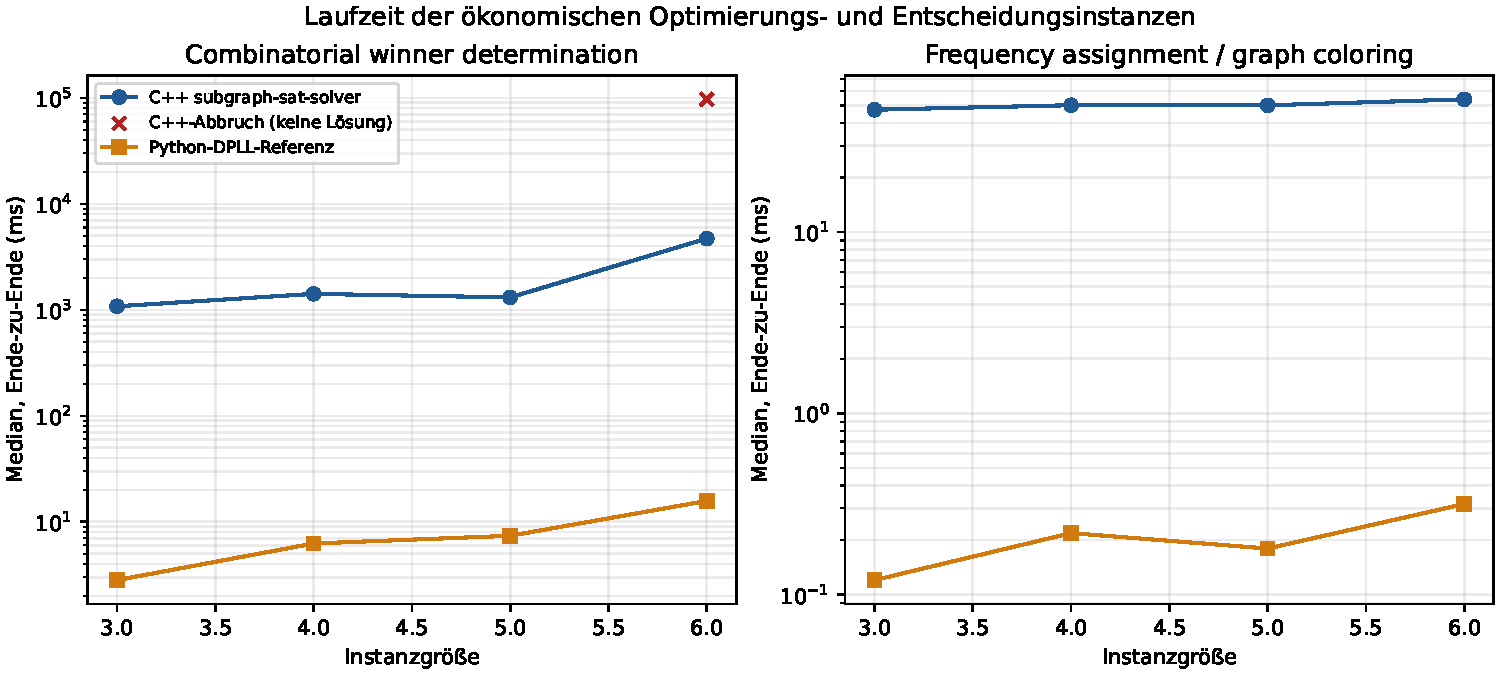
\includegraphics[width=0.92\textwidth]{../src/results/experiment_runtime.pdf}
\caption{Median der Ende-zu-Ende-Laufzeit in den gemessenen Auktionen und Repacking-Instanzen. Das Kreuz kennzeichnet einen abgebrochenen nativen Lauf.}
\label{fig:eco-experiment-runtime}
\end{figure}

\begin{figure}[ht]
\centering
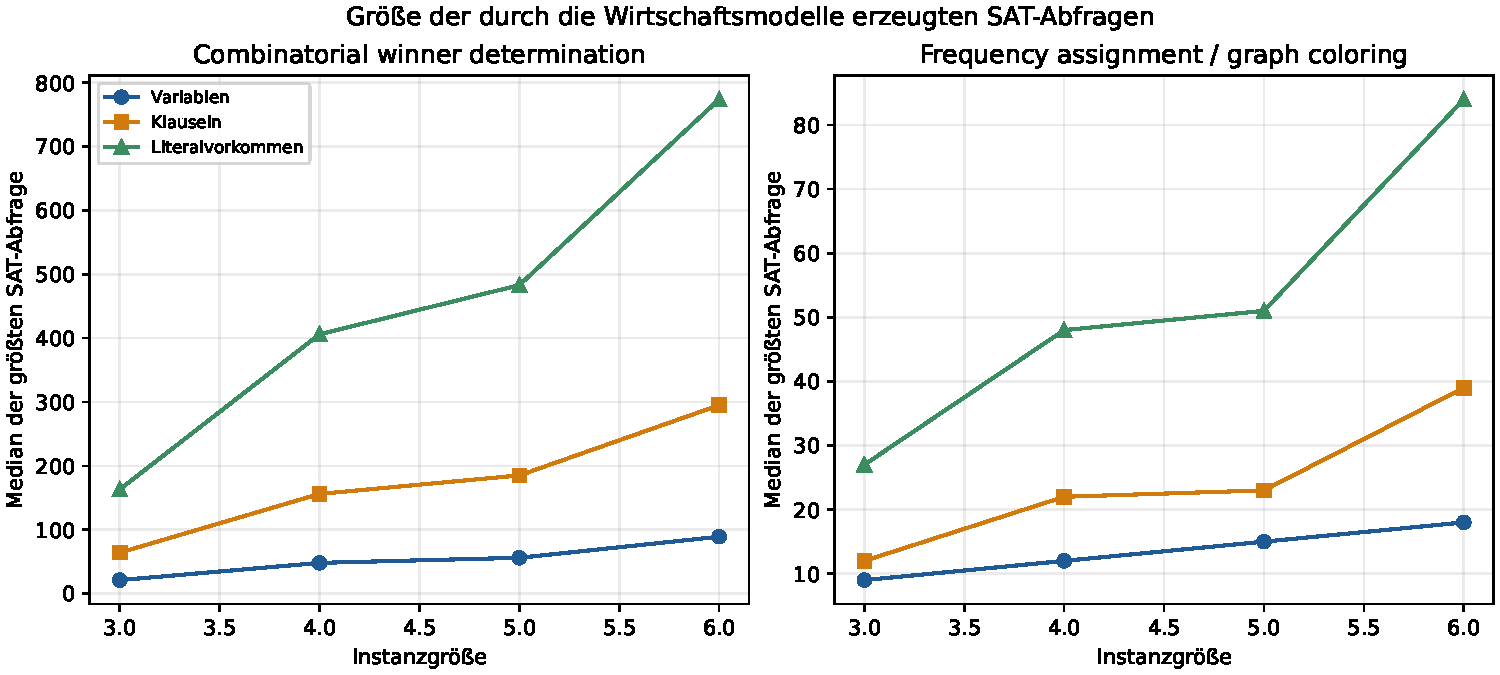
\includegraphics[width=0.92\textwidth]{../src/results/experiment_formula_size.pdf}
\caption{Größe der größten SAT-Abfrage je Instanz, gemessen in Variablen, Klauseln und Literalvorkommen.}
\label{fig:eco-experiment-cnf}
\end{figure}

Abbildung~\ref{fig:eco-experiment-phases} zerlegt die gemessene Arbeit des nativen Solvers nach den von ihm berichteten Phasen. Diese Werte summieren sich über die SAT-Aufrufe einer ökonomischen Optimierung. Sie sind daher nicht direkt mit der Laufzeit eines einzelnen SAT-Aufrufs gleichzusetzen; der äußere Ende-zu-Ende-Wert enthält außerdem Python-Modellierung, ctypes-Übergänge und Selbstreduktion.

\begin{figure}[ht]
\centering
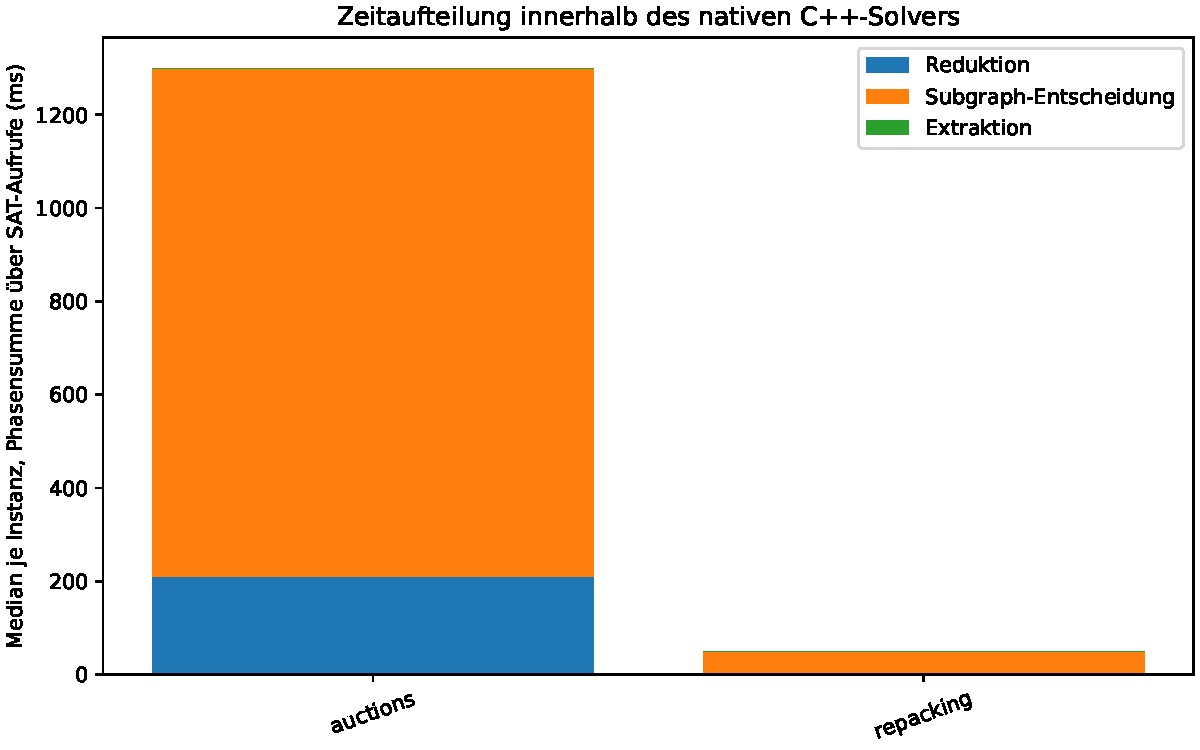
\includegraphics[width=0.7\textwidth]{../src/results/experiment_native_phases.pdf}
\caption{Median der aufsummierten nativen Reduktions-, Subgraph- und Extraktionszeiten je erfolgreicher Instanz.}
\label{fig:eco-experiment-phases}
\end{figure}

Abbildung~\ref{fig:eco-experiment-completion} ergänzt die Laufzeitgrafik um die Abschlussquote: Bei Auktionen wurden \(11\) von \(12\) nativen Fällen abgeschlossen, bei Repacking \(12\) von \(12\). Alle Rohmessungen einschließlich Seeds, Instanzgrößen, Zielfunktionswerten, Aufrufzahlen, CNF-Größen und nativen Phasenzeiten sind einzeln als JSON unter \texttt{src/results/} abgelegt. Die Abbildungen werden aus diesen Daten durch \texttt{src/experiments.py} mit Matplotlib erzeugt.

\begin{figure}[ht]
\centering
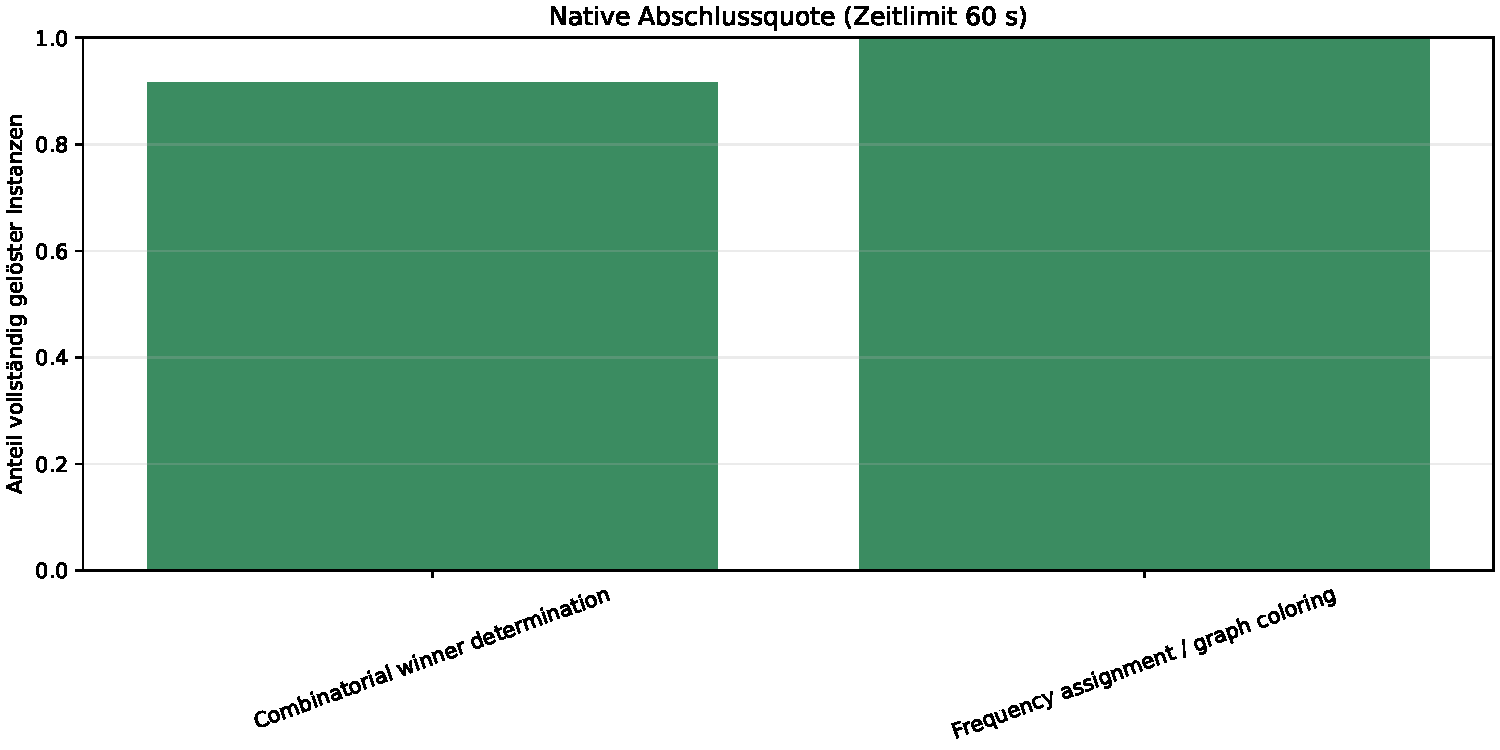
\includegraphics[width=0.85\textwidth]{../src/results/experiment_completion.pdf}
\caption{Anteil der nativen Instanzläufe mit vollständig zurückgegebenem Ergebnis (Zeitlimit je Subgraph-Entscheidung: 60 Sekunden).}
\label{fig:eco-experiment-completion}
\end{figure}

Die Messungen wurden unter Windows 11 mit Python 3.13.16, dem MinGW-C++-Compiler und den benachbarten Checkouts von \texttt{subgraph-sat-solver} und \texttt{csubgraph} ausgeführt. Die Instanzen sind durch feste Seeds reproduzierbar; Hardwaremodell und weitere Systemlast sind in den Ergebnisdateien jedoch nicht dokumentiert. Die Laufzeiten sind daher als Messwerte dieser konkreten Umgebung und nicht als universelle Kennzahlen zu lesen. Der native Pfad lief im exakten Modus; die unabhängige Referenz war der Python-DPLL aus dem Repository, kein optimierter CDCL-Solver.

Reproduktion aus dem Repository-Wurzelverzeichnis:
\begin{lstlisting}[language=bash]
python -m pip install -e .
python -m src.experiments --seed 20261013 --repetitions 3 --timeout-sec 60
\end{lstlisting}
Der Lauf baut den Shim gegen den benachbarten Checkout \texttt{../subgraph-sat-solver} und erwartet \texttt{../csubgraph/build/subgraph.exe}; alternative Orte sind über \texttt{--solver-dir} und \texttt{--subgraph-binary} angebbar. Jede abgeschlossene Instanz wird sofort in ihrer JSON-Datei gespeichert. Ein Timeout wird als Fehler protokolliert und nicht in UNSAT umgedeutet. Der vollständige Lauf erzeugt JSON-Dateien pro Familie und die PDF-Abbildungen unter \texttt{science/figures/}; nicht durchgeführte Familien dürfen dabei nicht als gemessene Resultate interpretiert werden.

\subsection{Interpretation und Grenzen}
Die Ergebnisse sind eine technische Machbarkeits- und Kostenaufnahme für zwei Modulbeispiele, keine repräsentative ökonomische Stichprobe. Vier der vorgesehenen Problemfamilien fehlen noch, die Fallzahlen pro Größe betragen nur drei, und die Auktionen zeigen bereits einen Timeout sowie stark streuende Laufzeiten. Weder lässt sich daraus auf große Märkte extrapolieren noch ein allgemeiner Leistungsvergleich von C++ und Python ableiten. Insbesondere belegen die Messungen nicht die Effizienzhypothese \(\Epoly\) oder eine polynomielle Laufzeit des Subgraph-Orakels. Ihr positiver Befund ist enger: Für 23 erfolgreich abgeschlossene synthetische Instanzen stimmen der native Solver und DPLL im Optimalwert überein, und die ausgegebenen Lösungen sind in den getesteten Modulen zulässig. Zugleich macht der hohe Anteil der Subgraph-Phase die Prozess- und Suchkosten des aktuellen nativen Integrationspfads sichtbar.

%%% ===================================================================
\section{Grenzen, Messplan und Fazit}
\label{eco:limits}

Tabelle \ref{tab:grenzen} fasst die Reichweite der Ergebnisse zusammen. Die Spalte „Problemklasse“ nennt die Komplexitätsklasse, die Spalte „Beispiel“ ein ökonomisches Problem, das in dieser Klasse liegt, und die Spalte „Wirkung von \(\Epoly\)“ beschreibt, ob und wie die Annahme \(\Epoly\) das Problem beeinflusst. Die Tabelle ist nicht erschöpfend; sie zeigt exemplarisch, dass \(\Epoly\) alle Probleme in \cNP{} und der Polynomialzeithierarchie betrifft, aber nicht Zähl- und \cPSPACE-Probleme, Informationsprobleme oder kryptographische Aufgaben.

\begin{table}[ht]
\centering\small
\begin{tabular}{p{4.3cm}p{3.4cm}p{6.2cm}}
\toprule
Problemklasse & Beispiel & Wirkung von \(\Epoly\)\\
\midrule
\cNP{} / \cCoNP & WDP, Repacking, Planung & polynomiell (Satz~\ref{satz:opt}, Kor.~\ref{kor:wop})\\
\(\Sigma_k^p,\Pi_k^p\) & robuste Mehrstufenplanung & polynomiell (Satz~\ref{satz:PH})\\
\cPPAD{} $\subseteq\cFNP$ & Nash-Näherung & polynomiell (Satz~\ref{satz:eps-nash})\\
\sharpP & Modell- und Gleichgewichtszählen & keine bekannte Wirkung (Satz~\ref{satz:sharpP})\\
\cPSPACE & POMDP, Spiele & keine bekannte Wirkung\\
Informationsprobleme & Hayek, Elicitation & keine Wirkung (Satz~\ref{satz:comm})\\
Kryptographie & Signaturen, Zahlungen & Zusammenbruch im asymptotischen Modell (Satz~\ref{satz:owf})\\
\bottomrule
\end{tabular}
\caption{Reichweite und Grenzen der Ergebnisse.}\label{tab:grenzen}
\end{table}

\subsection{Messplan mit dem Repository}
Die Ergebnisse sind konditional; empirisch lässt sich prüfen, wie weit die Kette praktisch trägt. Vorgeschlagen: (1) Auktionsinstanzen mit dem Generator CATS \cite{leytonbrown2000} und Repacking-Instanzen erzeugen, nach Satz~\ref{satz:wdp-sat} bzw. \ref{satz:repack} als DIMACS-CNF kodieren und an den Solver übergeben; (2) jede Antwort gegen einen unabhängigen Entscheider (CDCL, \cite{minisat}) und per Belegungsprüfung validieren; (3) Phasenlaufzeiten (Kodierung, Reduktion, Orakel, Extraktion), Zeitüberschreitungen und Fehler getrennt berichten; (4) Skalierung der Graphgröße gegen \(N^3\) (Lemma~\ref{lem:S3}) auftragen. Ein exaktes Ergebnis darf nur gemeldet werden, wenn der Orakelmodus exakt ist (Grundarbeit, Abschnitt zur Orakel-Schnittstelle). Die hier angegebenen Kodierungen (Auktion, Planung, Repacking, Standort, Rangaggregation, Pareto-Algorithmus) wurden vom Verfasser an kleinen Zufallsinstanzen gegen vollständige Enumeration geprüft; das ersetzt keine Beweise, sichert aber die Formeln.

\subsection{Fazit}
Unter der Annahme eines exakten, effizienten SAT-Entscheiders lösen sich in Polynomialzeit alle ökonomischen Entscheidungsprobleme in \cNP{} und der gesamten Polynomialzeithierarchie, einschließlich Auktionsauswertung, VCG-Zahlungen, Planung, Konfiguration und Gleichgewichtsberechnung. Nicht gelöst werden Zähl- und \cPSPACE-Probleme sowie Informations- und Anreizprobleme; und die kryptographische Grundlage digitaler Märkte bräche weg. Da die Annahme \(\cP=\cNP\) entspricht, sind die Kapitel als präzise Beschreibung des Szenarios zu lesen, nicht als Nachweis, dass der Solver es herbeiführt.

%%% END BODY

\begin{thebibliography}{99}
\bibitem{cook} S. A. Cook. The complexity of theorem-proving procedures. \emph{Proc. 3rd ACM STOC}, 1971.
\bibitem{karp} R. M. Karp. Reducibility among combinatorial problems. 1972.
\bibitem{papadimitriou} C. H. Papadimitriou. \emph{Computational Complexity}. Addison-Wesley, 1994.
\bibitem{arorabarak} S. Arora, B. Barak. \emph{Computational Complexity: A Modern Approach}. Cambridge University Press, 2009.
\bibitem{fortnow2009} L. Fortnow. The status of the P versus NP problem. \emph{CACM} 52(9):78--86, 2009.
\bibitem{aaronson2016} S. Aaronson. P $\overset{?}{=}$ NP. In: \emph{Open Problems in Mathematics}, Springer, 2016, 1--122.
\bibitem{valiant1979} L. G. Valiant. The complexity of enumeration and reliability problems. \emph{SIAM J. Comput.} 8(3):410--421, 1979.
\bibitem{stockmeyer1983} L. Stockmeyer. The complexity of approximate counting. \emph{STOC} 1983, 118--126.
\bibitem{papadimitriou1987} C. H. Papadimitriou, J. N. Tsitsiklis. The complexity of Markov decision processes. \emph{Math. Oper. Res.} 12(3):441--450, 1987.
\bibitem{simon1955} H. A. Simon. A behavioral model of rational choice. \emph{Quarterly J. Economics} 69(1):99--118, 1955.
\bibitem{rothkopf1998} M. H. Rothkopf, A. Pekeč, R. M. Harstad. Computationally manageable combinational auctions. \emph{Management Science} 44(8):1131--1147, 1998.
\bibitem{sandholm2002} T. Sandholm. Algorithm for optimal winner determination in combinatorial auctions. \emph{Artificial Intelligence} 135(1--2):1--54, 2002.
\bibitem{vickrey1961} W. Vickrey. Counterspeculation, auctions, and competitive sealed tenders. \emph{J. Finance} 16(1):8--37, 1961.
\bibitem{clarke1971} E. H. Clarke. Multipart pricing of public goods. \emph{Public Choice} 11:17--33, 1971.
\bibitem{groves1973} T. Groves. Incentives in teams. \emph{Econometrica} 41(4):617--631, 1973.
\bibitem{nisansegal2006} N. Nisan, I. Segal. The communication requirements of efficient allocations and supporting prices. \emph{J. Economic Theory} 129(1):192--224, 2006.
\bibitem{ausubelmilgrom2006} L. M. Ausubel, P. Milgrom. The lovely but lonely Vickrey auction. In: \emph{Combinatorial Auctions}, MIT Press, 2006.
\bibitem{nisanronen2001} N. Nisan, A. Ronen. Algorithmic mechanism design. \emph{Games and Economic Behavior} 35(1--2):166--196, 2001.
\bibitem{newman2018} N. Newman, A. Fréchette, K. Leyton-Brown. Deep optimization for spectrum repacking. \emph{CACM} 61(1):97--104, 2018.
\bibitem{frechette2016} A. Fréchette, N. Newman, K. Leyton-Brown. Solving the station repacking problem. \emph{AAAI} 2016.
\bibitem{abraham2007} D. J. Abraham, A. Blum, T. Sandholm. Clearing algorithms for barter exchange markets: Enabling nationwide kidney exchanges. \emph{ACM EC} 2007.
\bibitem{lenstra1977} J. K. Lenstra, A. H. G. Rinnooy Kan, P. Brucker. Complexity of machine scheduling problems. \emph{Annals of Discrete Mathematics} 1:343--362, 1977.
\bibitem{sinz2003} C. Sinz, A. Kaiser, W. Küchlin. Formal methods for the validation of automotive product configuration data. \emph{AI EDAM} 17(1):75--97, 2003.
\bibitem{bienstock1996} D. Bienstock. Computational study of a family of mixed-integer quadratic programming problems. \emph{Math. Programming} 74:121--140, 1996.
\bibitem{nash1951} J. Nash. Non-cooperative games. \emph{Annals of Mathematics} 54(2):286--295, 1951.
\bibitem{daskalakis2009} C. Daskalakis, P. W. Goldberg, C. H. Papadimitriou. The complexity of computing a Nash equilibrium. \emph{SIAM J. Comput.} 39(1):195--259, 2009.
\bibitem{chen2009} X. Chen, X. Deng, S.-H. Teng. Settling the complexity of computing two-player Nash equilibria. \emph{J. ACM} 56(3), 2009.
\bibitem{papadimitriou1994b} C. H. Papadimitriou. On the complexity of the parity argument and other inefficient proofs of existence. \emph{JCSS} 48(3):498--532, 1994.
\bibitem{megiddo1991} N. Megiddo, C. H. Papadimitriou. On total functions, existence theorems and computational complexity. \emph{Theoret. Comput. Sci.} 81(2):317--324, 1991.
\bibitem{gilboa1989} I. Gilboa, E. Zemel. Nash and correlated equilibria: Some complexity considerations. \emph{Games and Economic Behavior} 1:80--93, 1989.
\bibitem{conitzer2008} V. Conitzer, T. Sandholm. New complexity results about Nash equilibria. \emph{Games and Economic Behavior} 63(2):621--641, 2008.
\bibitem{schoenebeck2006} G. Schoenebeck, S. Vadhan. The computational complexity of Nash equilibria in concisely represented games. \emph{ACM EC} 2006, 270--279.
\bibitem{bartholdi1989a} J. Bartholdi, C. Tovey, M. Trick. Voting schemes for which it can be difficult to tell who won the election. \emph{Social Choice and Welfare} 6(2):157--165, 1989.
\bibitem{bartholdi1989b} J. Bartholdi, C. Tovey, M. Trick. The computational difficulty of manipulating an election. \emph{Social Choice and Welfare} 6(3):227--241, 1989.
\bibitem{gibbard1973} A. Gibbard. Manipulation of voting schemes. \emph{Econometrica} 41(4):587--601, 1973.
\bibitem{satterthwaite1975} M. Satterthwaite. Strategy-proofness and Arrow's conditions. \emph{J. Economic Theory} 10(2):187--217, 1975.
\bibitem{impagliazzoluby1989} R. Impagliazzo, M. Luby. One-way functions are essential for complexity based cryptography. \emph{FOCS} 1989.
\bibitem{impagliazzo1995} R. Impagliazzo. A personal view of average-case complexity. \emph{Structure in Complexity Theory} 1995, 134--147.
\bibitem{goldreich2001} O. Goldreich. \emph{Foundations of Cryptography, Vol. I}. Cambridge University Press, 2001.
\bibitem{shannon1949} C. E. Shannon. Communication theory of secrecy systems. \emph{Bell System Technical J.} 28(4):656--715, 1949.
\bibitem{hayek1945} F. A. Hayek. The use of knowledge in society. \emph{American Economic Review} 35(4):519--530, 1945.
\bibitem{mises1920} L. von Mises. Die Wirtschaftsrechnung im sozialistischen Gemeinwesen. \emph{Archiv für Sozialwissenschaften} 47:86--121, 1920.
\bibitem{hurwicz1972} L. Hurwicz. On informationally decentralized systems. In: \emph{Decision and Organization}, North-Holland, 1972.
\bibitem{khachiyan1979} L. G. Khachiyan. A polynomial algorithm in linear programming. \emph{Soviet Math. Doklady} 20:191--194, 1979.
\bibitem{coase1937} R. H. Coase. The nature of the firm. \emph{Economica} 4(16):386--405, 1937.
\bibitem{leytonbrown2000} K. Leyton-Brown, M. Pearson, Y. Shoham. Towards a universal test suite for combinatorial auction algorithms. \emph{ACM EC} 2000, 66--76.
\bibitem{minisat} N. Eén, N. Sörensson. An extensible SAT-solver. \emph{SAT 2003}, 502--518.
\end{thebibliography}
\end{document}
